\documentclass[11pt]{article}
\usepackage[margin=1.1in]{geometry}
\usepackage{amsmath}
\usepackage{amsthm}
\newtheorem{proposition}{Proposition}
\newtheorem{corollary}{Corollary}
\usepackage{booktabs}
\usepackage{microtype}
\usepackage{tikz}
\usepackage{float}
\usepackage[colorlinks=true,allcolors=blue]{hyperref}

\title{\textbf{Softmax Masking Is a Transport Assumption:\\Evidence from Thirty-Nine Tests of Linear\\versus Gaussian Renormalization}}
\author{Peter Cotton}
\date{Provisional draft, 31 August 2026}

\begin{document}
\maketitle

\begin{abstract}
\noindent Re-scaling a probability vector when an item is withdrawn, delisted or masked out is
one of the great unconscious modelling acts. When the support shrinks because something was
learned about a fixed experiment, that re-scaling is the conditional law and there is nothing to
choose. When instead somebody intervenes on what may be chosen, the old vector does not determine
the new one, and re-scaling amounts to assuming a Gumbel distribution within the additive
random-utility class\footnotemark[6]. A Gaussian is an equally canonical and equally tuning-free
choice. We call the latter \emph{Gaussian renormalization} and set it alongside linear, or
proportional, renormalization in a two horse empirical race, which is fair because neither carries
a parameter fitted to the data being predicted. In part we re-litigate the psychology debate that
sets the constant ratio rule, Luce's choice axiom, against Thurstone's Case V; in part we bring
new data from situations where renormalizing a probability is tempting. Gaussian renormalization
has the lower held-out log loss in thirty of thirty-nine comparisons. The differences are small
where they are small, a median of $0.004$ nats across all thirty-nine, and twelve exceed $0.01$
with a maximum of $0.05$.
\end{abstract}

\footnotetext[6]{The Gumbel construction is due to Holman and Marley
\cite{lucesuppes1965,holman1974}; the uniqueness is Yellott's \cite{yellott1977}.}

\section{A two horse race between zero parameter choice models}
\label{sec:problem}

Suppose a probability vector is presented, as with a collection of de-vigged bookmaker odds for a
horse race, or the output of a calibrated probabilistic machine learning model. Suppose next that
the set changes. Perhaps a horse is scratched, a product is delisted, or a primary candidate
drops out of a race. Alternatively a response option in a survey may be disallowed, or a token
masked out of a softmax. These are quite different situations with their own nuances, but in each
case a probability vector has to be transported from the original support to a smaller one. The
natural question arises: what are the probabilities over what remains?

The question is only open in some of them, and the arithmetic does not tell you which. Suppose the
probability vector describes a fixed experiment and we learn that the outcome fell in $T$. Then
$p_i / \sum_{j \in T} p_j$ is the conditional law by definition, and there is nothing to choose.
Masking a fixed softmax and rescaling the survivors performs that same arithmetic on a score
vector, so wherever the target really is the conditional law, that operation is right by
construction and this paper does not bear on it. A third case is a model that recomputes its
scores with the permitted set as an input; its output is not a transport of the old vector at
all, and neither map below describes it.

What is left is the case this paper is about. Somebody intervenes on the feasible set. The horse
is scratched, the option is disallowed, the action is removed, and the experiment that generates
the choice is not the one that generated the shares. The old vector does not determine the new
one, and any answer is a modelling assumption. The same masking arithmetic is often applied here
too, and that is where it stops being a theorem and starts being a choice.

Writing $Y(S)$ for what a chooser facing menu $S$ selects, and $P_S(i) = \Pr\{Y(S) = i\}$ for the
share it produces, the four separate:
\begin{center}
\small
\begin{tabular}{lll}
\toprule
Operation & Target & Status \\
\midrule
Outcome information & $\Pr\{Y(S) = i \mid Y(S) \in T\}$ & linear by definition \\
Mask on a fixed score vector & the same quantity, computed & linear by construction \\
Feasible-set intervention & $P_T(i)$ & not identified by $P_S$ \\
Menu-aware recomputation & $P_T(i)$, estimated directly & no transport needed \\
\bottomrule
\end{tabular}
\end{center}
The first two condition the law of $Y(S)$; the third asks about $Y(T)$, a different random
variable produced by a different experiment, and that is what $P_S$ alone cannot determine. We
write $P_S(i)$ rather than $P(i \mid S)$ throughout, because the conditioning bar is exactly the
confusion at issue.

A related problem arises in the computation of permutation probabilities, but here we focus on
the case where the original vector is a market share of sorts, as with the population popularity
of an item on a menu. That data is the more controversial in some respects, because it can speak
to the discovery or delineation of underlying mechanics from revealed preferences. In contrast it
is somewhat self-evident that the right answer for contest winning probabilities can often be
strongly suggested by the generative model at hand, finishing time distributions being the
obvious example.

When a menu item is removed, quite a lot of machinery exists for carefully estimating the
probabilities that should be ascribed to the reduced menu. Depending on the data available,
probit models or other tools can be brought to bear. That is outside the scope of the present
discussion, because wielding statistical machinery together with careful modelling, parameter
selection and cross-validation can evolve into an entire enterprise, and it is often unreasonable
to compare that to the trivial, instinctive act of rescaling probability. That reflex cannot be
challenged by an invitation to treat every occasion for its use as a new data science project.

There is one alternative response that is slightly more involved analytically but not
methodologically complicated. It is the Gaussian special case of Thurstone's Case V family, and
we argue for its place as a tuning-free default renormalization to set against the linear one.
Both stand on equal footing philosophically.

Nothing has been observed about the smaller menu, so the answer must come from an assumption
about how the original shares arose. The standard rescaling assumption is stated by Luce's axiom
\cite{luce1959}, which assigns each item $i$ on menu $S$ a worth $u(i)$ with
\begin{equation}
p_i = \frac{u(i)}{\sum_{j \in S} u(j)},
\label{eq:luce}
\end{equation}
so the shares determine the worths up to scale. The prediction for a subset $T \subseteq S$
follows by changing the denominator alone, which leaves every ratio $p_i/p_j$ with $i,j \in T$
as it was in $S$. For a two-item menu the predicted share preferring $i$ is $p_i/(p_i+p_j)$.
This is proportional, or \emph{linear}, renormalization. The invariance it imposes is Independence of Irrelevant
Alternatives, and applied to a reduced set of response alternatives it is what Clarke
\cite{clarke1957} named the \emph{constant-ratio rule}.

We suggest that Gaussian renormalization is equally natural, if not more so. Read the shares as
the winning probabilities of a contest among independent Gaussian performances, which has
heritage back to Thurstone's Case V \cite{thurstone1927} generalized from pairs to a multiway
field. Item $i$
carries a location $a_i$, draws $X_i \sim N(a_i,1)$ on each occasion, and the highest draw is
chosen, so
\begin{equation}
p_i = \int \varphi(x - a_i) \prod_{k \neq i} \Phi(x - a_k)\, dx.
\label{eq:winprob}
\end{equation}
Given the shares, this is inverted for the locations, which are identified up to a common
translation and fixed here by $\sum_i a_i = 0$. The prediction for a subset $T$ is the same
contest run among $T$ alone. For a pair it is one normal evaluation,
\begin{equation}
P(X_i > X_j) = \Phi\!\left(\frac{a_i - a_j}{\sqrt{2}}\right).
\label{eq:pair}
\end{equation}

Our limited goal is a practical comparison of linear renormalization and Gaussian
renormalization. Neither carries a parameter fitted to the data being predicted, which is the
sense in which both are free of tuning; the pipeline around them does use one shared convention,
the continuity correction $\alpha = 1/2$, and Section~\ref{sec:conventions} varies it.
The first holds the ratios of the shares fixed, the second holds the latent
locations fixed. The underlying physics is quite different, so even small persistent statistical
advantages of one over the other may be suggestive of structure, and of interest to the
psychology community but also, we hope, to the broader machine learning audience whose choice of
linear renormalization is often tacit.

Each competitor in this two horse race is elementary and, not surprisingly, has assumed many
names. We treat them as synonyms. We equate proportional renormalization, linear renormalization,
the ratio rule, Clarke's constant-ratio rule, and masking a softmax and rescaling the survivors.
All denote Equation~\eqref{eq:luce} applied to a subset, and we write linear renormalization
except where the historical name is what a cited paper used.

Conversely we equate Gaussian renormalization, Thurstone's Case V re-run among the survivors, and
the independent unit-variance Gaussian contest on the restricted menu. The names differ by
discipline and by decade rather than by content, and part of why the comparison we present has
not been made broadly or crisply is that the two literatures holding the pieces did not share a
vocabulary.

The two horses disagree, and in a fixed direction. If $p_i > p_j$ then Equation~\eqref{eq:pair}
lies between $\tfrac12$ and the renormalized $p_i/(p_i+p_j)$: winning a large field requires an
unusually high draw and beating a single rival does not, so withdrawing the other alternatives
counts the favourite's advantage for less. Section~\ref{sec:maps} remarks that these two are the
conventional members of the independent additive random-utility class, which is well appreciated,
and Proposition~\ref{prop:contraction} makes the direction of their disagreement exact.

\section{Scoreboard}

Lest we be accused of burying the lead, Figure~\ref{fig:line} and Table~\ref{tab:scoreboard} come
first. They are aimed at anyone whose strong inclination is Luce's choice axiom, and in
particular at the impression that dividing probabilities is an argument in itself.

The figure asks where each population falls between the two kinds of renormalization, on a scale
where linear renormalization is one point and Gaussian renormalization another. Of the twenty it
can place, nineteen lie nearer the Gaussian point, the median sits at $1.16$, and fifteen lie
beyond it.

The single population nearer linear renormalization comes from one experiment in which subjects
chose among gambles whose values had to be computed, which takes on a bit of the flavour of a quiz
and so might be classified separately. The figure is suggestive rather than decisive, since the
statistic it plots is not a proper scoring rule and its ratio is unstable where the Case V slope
is small.

The table is the defensible version of the same comparison, and what it refutes is the notion that
linear renormalization has any natural advantage, or should occupy the special place that in
practice it tends to claim. Thirty-nine comparisons have full-menu shares that
calibrate both maps and restricted-menu choices. The score is held-out log loss.

Another caveat: rows are comparisons. Several reuse the same subjects or source study, so they are
not to be considered independent tests of the same hypothesis. Section~\ref{sec:empirical} goes
into complete detail on the protocol, the datasets and the null.

\begin{figure}[H]
\centering
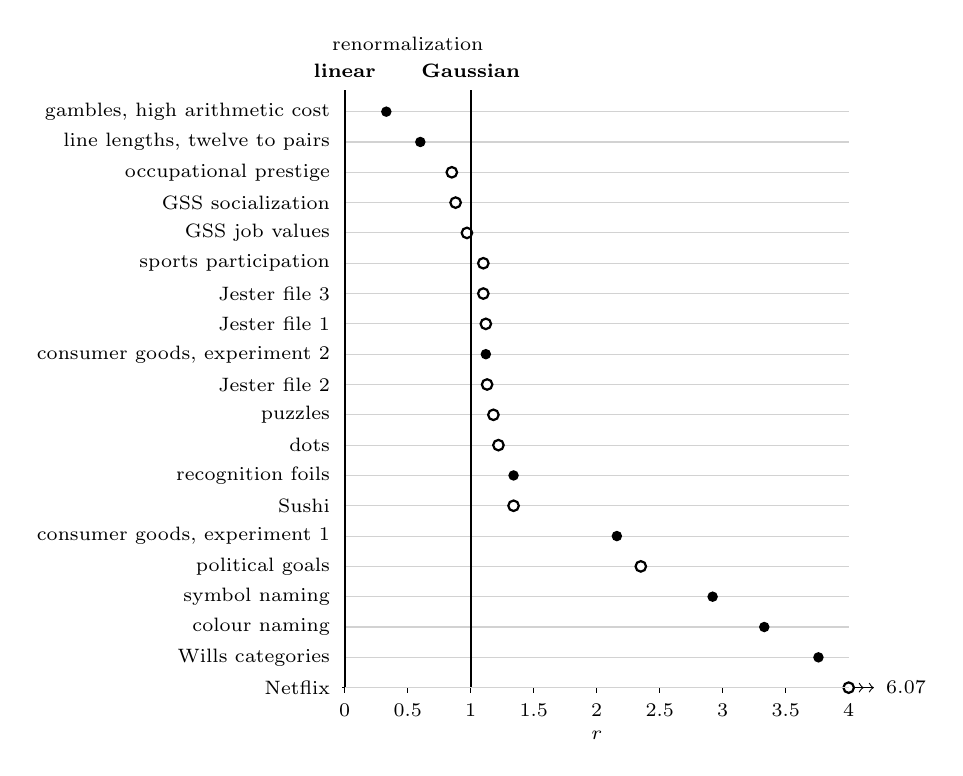
\begin{tikzpicture}[x=1.6cm,y=0.385cm]
  \node[font=\scriptsize,anchor=east] at (-0.04,0) {gambles, high arithmetic cost};
  \draw[gray!35,thin] (0,0) -- (4.0,0);
  \fill (0.33,0) circle (1.9pt);
  \node[font=\scriptsize,anchor=east] at (-0.04,-1) {line lengths, twelve to pairs};
  \draw[gray!35,thin] (0,-1) -- (4.0,-1);
  \fill (0.60,-1) circle (1.9pt);
  \node[font=\scriptsize,anchor=east] at (-0.04,-2) {occupational prestige};
  \draw[gray!35,thin] (0,-2) -- (4.0,-2);
  \draw[fill=white,thick] (0.85,-2) circle (1.9pt);
  \node[font=\scriptsize,anchor=east] at (-0.04,-3) {GSS socialization};
  \draw[gray!35,thin] (0,-3) -- (4.0,-3);
  \draw[fill=white,thick] (0.88,-3) circle (1.9pt);
  \node[font=\scriptsize,anchor=east] at (-0.04,-4) {GSS job values};
  \draw[gray!35,thin] (0,-4) -- (4.0,-4);
  \draw[fill=white,thick] (0.97,-4) circle (1.9pt);
  \node[font=\scriptsize,anchor=east] at (-0.04,-5) {sports participation};
  \draw[gray!35,thin] (0,-5) -- (4.0,-5);
  \draw[fill=white,thick] (1.10,-5) circle (1.9pt);
  \node[font=\scriptsize,anchor=east] at (-0.04,-6) {Jester file 3};
  \draw[gray!35,thin] (0,-6) -- (4.0,-6);
  \draw[fill=white,thick] (1.10,-6) circle (1.9pt);
  \node[font=\scriptsize,anchor=east] at (-0.04,-7) {Jester file 1};
  \draw[gray!35,thin] (0,-7) -- (4.0,-7);
  \draw[fill=white,thick] (1.12,-7) circle (1.9pt);
  \node[font=\scriptsize,anchor=east] at (-0.04,-8) {consumer goods, experiment 2};
  \draw[gray!35,thin] (0,-8) -- (4.0,-8);
  \fill (1.12,-8) circle (1.9pt);
  \node[font=\scriptsize,anchor=east] at (-0.04,-9) {Jester file 2};
  \draw[gray!35,thin] (0,-9) -- (4.0,-9);
  \draw[fill=white,thick] (1.13,-9) circle (1.9pt);
  \node[font=\scriptsize,anchor=east] at (-0.04,-10) {puzzles};
  \draw[gray!35,thin] (0,-10) -- (4.0,-10);
  \draw[fill=white,thick] (1.18,-10) circle (1.9pt);
  \node[font=\scriptsize,anchor=east] at (-0.04,-11) {dots};
  \draw[gray!35,thin] (0,-11) -- (4.0,-11);
  \draw[fill=white,thick] (1.22,-11) circle (1.9pt);
  \node[font=\scriptsize,anchor=east] at (-0.04,-12) {recognition foils};
  \draw[gray!35,thin] (0,-12) -- (4.0,-12);
  \fill (1.34,-12) circle (1.9pt);
  \node[font=\scriptsize,anchor=east] at (-0.04,-13) {Sushi};
  \draw[gray!35,thin] (0,-13) -- (4.0,-13);
  \draw[fill=white,thick] (1.34,-13) circle (1.9pt);
  \node[font=\scriptsize,anchor=east] at (-0.04,-14) {consumer goods, experiment 1};
  \draw[gray!35,thin] (0,-14) -- (4.0,-14);
  \fill (2.16,-14) circle (1.9pt);
  \node[font=\scriptsize,anchor=east] at (-0.04,-15) {political goals};
  \draw[gray!35,thin] (0,-15) -- (4.0,-15);
  \draw[fill=white,thick] (2.35,-15) circle (1.9pt);
  \node[font=\scriptsize,anchor=east] at (-0.04,-16) {symbol naming};
  \draw[gray!35,thin] (0,-16) -- (4.0,-16);
  \fill (2.92,-16) circle (1.9pt);
  \node[font=\scriptsize,anchor=east] at (-0.04,-17) {colour naming};
  \draw[gray!35,thin] (0,-17) -- (4.0,-17);
  \fill (3.33,-17) circle (1.9pt);
  \node[font=\scriptsize,anchor=east] at (-0.04,-18) {Wills categories};
  \draw[gray!35,thin] (0,-18) -- (4.0,-18);
  \fill (3.76,-18) circle (1.9pt);
  \draw[thick] (0,0.7) -- (0,-19.00);
  \draw[thick] (1,0.7) -- (1,-19.00);
  \node[font=\scriptsize\bfseries,anchor=south] at (0,0.8) {linear};
  \node[font=\scriptsize\bfseries,anchor=south] at (1,0.8) {Gaussian};
  \node[font=\scriptsize,anchor=south] at (0.5,1.7) {renormalization};
  \draw[->] (-0.02,-19.00) -- (4.12,-19.00);
  \foreach \x in {0,0.5,1,1.5,2,2.5,3,3.5,4}
    {\draw ({\x},-19.00) -- ({\x},-19.18);
      \node[font=\scriptsize,anchor=north] at ({\x},-19.22) {\x};}
  \node[font=\scriptsize,anchor=north] at (2.0,-20.10) {$r$};
  \draw[fill=white,thick] (4.0,-19) circle (1.9pt);
  \node[font=\scriptsize,anchor=east] at (-0.04,-19) {Netflix};
  \draw[gray!35,thin] (0,-19) -- (4.0,-19);
  \draw[->] (4.05,-19) -- (4.2,-19);
  \node[font=\scriptsize,anchor=west] at (4.22,-19) {$6.07$};
\end{tikzpicture}
\caption{Where each population sits between the two maps. The coordinate is
$r = \lambda_{\text{observed}} / \lambda_{\text{Case V}}$, the observed contraction slope
divided by the slope Case V implies for that population's own shares, so linear renormalization
is at $r = 0$ by construction and Gaussian renormalization at $r = 1$. Filled circles are
restricted menus the observer actually faced, open circles are ranking-induced. Most populations
lie beyond $r = 1$: choice contracts by more than Case V predicts, so as a general observation
the Gaussian point tends not to be far enough along the family. A collection appears when a
restricted pairwise share $q_{ij}$ exists on the alternatives that calibrated the map, which
twenty of the thirty-nine comparisons have. The tone, Getty and Townsend rows restrict to sets of
three or more, so no $q_{ij}$ exists; the news, ballot and Wikipedia rows have no matched pair on
fixed alternatives. The ratio is ill-conditioned where the Case V slope is small, which is why
Netflix reaches $6.07$ on a Case V slope of $0.102$ while its held-out gain is $0.0009$; the
extremes of this axis are its least certain points. This statistic is not proper, so refer also
to Table~\ref{tab:scoreboard}, which does not order the populations the same way.}
\label{fig:line}
\end{figure}

Two numbers are reported for each population. The \emph{gain} is the held-out log loss of linear
renormalization minus that of Gaussian renormalization, in nats per prediction, so a positive gain
means Gaussian renormalization forecast the withheld choices better. The \emph{null frequency} is
obtained by generating a population that obeys the constant-ratio rule exactly, with worths set to
the observed shares, pushing it through the identical pipeline, and recording how often that
population produces a gain at least as large as the observed one. It is a parametric bootstrap
frequency under one particular joint law, Plackett--Luce for the ranking collections and
independent redraws for the menu experiment, and not a model-free test of the constant-ratio
restriction. It is reported as a diagnostic and should not be read as a $p$-value.

\begin{table}[!t]
\centering
\small
\begin{tabular}{llrrl}
\toprule
Population & Restriction & Gain & Null freq. & Family \\
\midrule
News slates & observed impressions & $+.0496$ & $.016$\footnotemark[7] & clicks \\
Sounds, eight to four, $\{1,3,5,7\}$ & observed menus & $+.0490$ & $\le .005$ & Getty \\
Sounds, eight to four, $\{1,2,5,6\}$ & observed menus & $+.0453$ & $\le .005$ & Getty \\
Consumer goods 1, forced choice & observed menus & $+.0442$ & $.005$ & Costa-Gomes \\
Occupational prestige & ranking-induced & $+.0391$ & $\le .005$ & prestige \\
Wills categories, three to two & observed menus & $+.0299$ & $.002$ & categorization \\
Symbol naming, six to two & observed menus & $+.0278$ & $\le .005$ & Yeon--Rahnev \\
Colour naming, four to two & observed menus & $+.0147$ & $\le .005$ & Yeon--Rahnev \\
Consumer goods 1, all subjects & observed menus & $+.0140$ & $.010$ & Costa-Gomes \\
Consumer goods 2, forced choice & observed menus & $+.0140$ & $.129$ & Costa-Gomes \\
Sushi & ranking-induced & $+.0111$ & $\le .005$ & preference \\
Gambles, high arithmetic cost & observed menus & $+.0101$ & $.035$ & Aguiar \\
Letters, five to three, $\{F,H,X\}$ & observed menus & $+.0093$ & $.005$ & Townsend--Landon \\
Political goals & ranking-induced & $+.0076$ & $\le .005$ & preference \\
Gambles, medium arithmetic cost & observed menus & $+.0068$ & $.124$ & Aguiar \\
Consumer goods 2, all subjects & observed menus & $+.0059$ & $.199$ & Costa-Gomes \\
GSS socialization & ranking-induced & $+.0057$ & $\le .005$ & GSS \\
Sports participation & ranking-induced & $+.0051$ & $.51$ & preference \\
Letters, five to three, $\{A,E,X\}$ & observed menus & $+.0040$ & $.010$ & Townsend--Landon \\
Recognition foils, four to two & observed menus & $+.0037$ & $\le .005$ & Utochkin \\
Jester file 3 & ranking-induced & $+.0024$ & $\le .005$ & Jester \\
Jester file 1 & ranking-induced & $+.0020$ & $\le .005$ & Jester \\
Jester file 2 & ranking-induced & $+.0018$ & $\le .005$ & Jester \\
GSS job values & ranking-induced & $+.0018$ & $\le .005$ & GSS \\
Dots & ranking-induced & $+.0016$ & $\le .005$ & perceptual \\
Netflix & ranking-induced & $+.0013$ & $\le .005$ & film \\
Puzzles & ranking-induced & $+.0008$ & $\le .005$ & perceptual \\
Letters, five to four, $\{A,E,F,H\}$ & observed menus & $+.0006$ & $.129$ & Townsend--Landon \\
US state ballots 2024 & observed ballots & $+.0002$ & $.005$ & ballots \\
Gambles, low arithmetic cost & observed menus & $+.0002$ & $.667$ & Aguiar \\
\midrule
Wikipedia links & observed removals & $-.0001$ & $.005$ & clicks \\
Tones, wide, ten to eight & observed menus & $-.0041$ & n/a & Stewart \\
Tones, narrow, ten to eight & observed menus & $-.0051$ & n/a & Stewart \\
Lines, twelve to eight & observed menus & $-.0057$ & $1.000$ & lines\footnotemark[8] \\
Lines, twelve to four & observed menus & $-.0090$ & $1.000$ & lines\footnotemark[8] \\
Sounds, eight to four, $\{3,4,5,6\}$ & observed menus & $-.0127$ & $1.000$ & Getty \\
Tones, narrow, ten to six & observed menus & $-.0133$ & n/a & Stewart \\
Tones, wide, ten to six & observed menus & $-.0173$ & n/a & Stewart \\
Lines, twelve to two & observed menus & $-.0322$ & $1.000$ & lines\footnotemark[8] \\
\bottomrule
\end{tabular}
\caption{Held-out log loss of linear renormalization minus that of Gaussian renormalization, in
nats per prediction. Here we read a positive gain as a win for Gaussian renormalization. The null
frequency is defined in the text. It is a parametric bootstrap diagnostic for departure from the
constant-ratio rule, not a $p$-value and not a statement about predictive superiority. Replicates are two hundred except for the news row, sixty, and the Wills
row, four hundred; the tone matrices are participant-averaged, so no null frequency is computed.}
\label{tab:scoreboard}
\end{table}

\footnotetext[7]{The news figure rests on sixty replicates, so $.016$ is the floor $1/61$ rather
than a measured frequency.}
\footnotetext[8]{The twelve-line data is unpublished laboratory data with no licence file and no
associated publication, so we do not attribute it to a named author. See the data section.}

Gaussian renormalization performs strongly. It has the lower held-out log loss in thirty of the
thirty-nine rows. That count is a description of this table and not an estimate of any rate,
because the rows are not independent and the families contribute unequal numbers of
them.\footnote{As a finer point, the collections were assembled by searching for restriction data.
It could be argued that this is therefore not a fair sample from a population of applications.}

We forward an explanation for eight of the nine rows where linear renormalization wins. Four are
tone identification and three are line identification. Another is the Getty condition whose four
surviving sounds are easily mistaken for one another. All three studies place the alternatives on
a single perceptual dimension, which is the obvious reading, though
Section~\ref{sec:boundary} treats them together and finds the dimension is not itself the cause.
The ninth is Wikipedia, whose magnitude is $-0.0001$.

The two columns answer different questions. A positive gain says Gaussian renormalization
predicted better from estimated shares, and part of that can be shrinkage rather than structure. A
small null frequency says the population departs from the constant-ratio rule in the direction of
contraction, and says nothing about which map forecasts better.

Two rows show the questions coming apart. Wikipedia has a negative gain and a small null
frequency, so it departs from the rule in the right direction while still predicting worse. Sports
participation has a positive gain and a null frequency of $0.51$, so its gain is shrinkage and it
carries no evidence about the rule. Section~\ref{sec:empirical} takes up the first question and
Section~\ref{sec:null} the second.

Each consumer experiment appears twice because a gain and a null frequency have to come from the
same people, and the forced-choice subgroup is not the whole sample. Three further populations
appear in Section~\ref{sec:boundary} instead of here, since published aggregates fix the direction
of their failure but do not support this protocol.

\section{Prior tests of the constant-ratio rule}
\label{sec:prior}

Some experiments have a very simple setup. A stimulus is presented that is supposed to be matched
to one of a fixed set of responses. Then the response list is reduced and the same experiment is
repeated. Each row of the resulting confusion matrix is the response distribution for one
stimulus, and the rule predicts the reduced matrix from the full one.

Clarke had listeners identify consonant-vowel syllables heard against noise, and obtained three
six-by-six master matrices together with six three-by-three submatrices drawn from them. Clarke
and Anderson \cite{clarkeanderson1957} repeated the test on a ten-item set using naive rather
than practised listeners, so that practice could be considered as a possible confound.

Pollack and Decker \cite{pollackdecker1960} used eight word-initial consonants in noise, with
three overlapping four-way subsets. They used different signal-to-noise ratios. They reported
average deviations near four per cent.

Hodge \cite{hodge1967} is similar in spirit but used lifted weights and visual size. An original
eight-item list was then cut to four, and then two. Rich \cite{rich1971} used a different kind of
imperfection, our short-term memory. Getty, Swets, Swets and Green \cite{getty1979} kept all
eight stimuli in play and cut only the permitted responses, to four at a time in three different
sets. Here nothing about the stimulus was changed.

Morgan \cite{morgan1974} built a likelihood-ratio test and rejected the constant-ratio rule on
the earlier data, which was a useful redirect for our own broader set of studies; see the
comparison between Figure~\ref{fig:line} and Table~\ref{tab:scoreboard}.

Townsend and Landon \cite{townsendlandon1982} ran one master set of five letters with three
nested response sets. They used a blocked and counterbalanced design. They published the full
matrices per subject.

Like us, Rouder \cite{rouder2004} concludes that conditioning on a reduced choice set
is better than a guessing correction predicts and worse than the ratio rule predicts.
Wills, Reimers, Stewart, Suret and McLaren \cite{wills2000} also reject the constant-ratio rule
in categorization and conclude that it should be replaced by a system based on Thurstonian
choice.

Their route to this was via a fitted
four-parameter winner-take-all model, and they also examine a parameter-free version that simply
picks the largest noisy magnitude. They say that Gaussian noise ``produces comparable results''
to the rectangular noise they use.

Their setting differs from this one in what is available at the outset. They have a model of the
stimulus, so their magnitudes are a function of how many category-appropriate symbols a display
contains, and a stimulus model of that kind motivates one noise law over another. Here there is
no stimulus, only a probability vector, and the noise law has to be chosen. Their Experiment 2
withdraws a response category and their trial data is deposited, so it is scored below with the
rest, where it agrees with them: Gaussian renormalization has the lower held-out loss by
$0.0299$ nats.

Three findings recur across those studies. The rule is a fair first approximation. It fails by
concentrating the withdrawn mass onto whichever survivor most resembles the removed alternative
rather than spreading it proportionally. Townsend and Landon attribute that to Debreu's
similarity objection, and Rouder brackets the same failure from the other side, finding real
behaviour better than a guessing correction predicts. And every claim of conformity that was later
retested with a test that had power was overturned. Holloway reversed his own 1968 conclusion in
1971 \cite{holloway1968,holloway1971}, and Morgan's likelihood-ratio test rejected the rule on
both of the datasets he applied it to, Clarke's and Egan's \cite{egan1957,morgan1974}.

The reason the question stayed open is stated in the literature itself. Clarke returned to it in
1959 with four kinds of signal ensemble and three competing models, and reported that ``the
simplified version of the constant-ratio rule and the simplified version of the theory of signal
detectability were both compatible with the data obtained in the speech experiments''
\cite{clarke1959}. The theory of signal detectability is the Gaussian account. So the two
candidates compared in this paper were already run against each other in 1959, and the verdict
was that percent correct could not separate them. The confusion matrices that would have
separated them were printed but never used for that purpose!

Clarke's 1959 abstract also records the boundary condition of
Section~\ref{sec:boundary}: ``No model tested was sufficiently
complex to account for data when the sinusoidal signals varied only in amplitude or only in
frequency''. Both accounts failed on unidimensional continua at the outset, which is where the
tone and line collections below place them.

The literature contains no comparison against a second assumption that also has no free
parameters. Lee \cite{lee1968} proposed one analytically, observing that detection
theory and the constant-ratio rule diverge most for unidimensional stimuli and that the gap
could serve in diagnosis, but did not carry it out on data. Nor was any of this scored out of
sample; the tests are goodness-of-fit statements about the matrix in hand.
Appendix~\ref{sec:census} is a census of one hundred and thirty-three sources, recording which of them printed
or deposited enough to score either assumption.

\section{Theory}
\label{sec:theory}

\subsection{Why these two maps}
\label{sec:maps}

Renormalization does not follow from probability theory. It is the correct posterior for
mutually exclusive events only when learning that one of them is impossible says nothing about
which of the rest obtained. Monty Hall is the familiar case where it does not: conditioning is
still correct there, but the host's choice of door carries more information than the bare fact
that the car is not behind it, so the event conditioned on is not simply $Y \in T$. Withdrawal is
neither of those two cases, because no information about a fixed experiment has arrived at all.
An alternative is gone, which is a different problem.
Conditioning requires a model of how the probabilities were generated, and linear renormalization supplies one.

Which model it supplies is known. Within the class of independent additive random-utility
models, Gumbel errors generate Equation~\eqref{eq:luce}
\cite{lucesuppes1965,holman1974}, and Yellott \cite{yellott1977} showed the noise law is
identified once menus of three or more are included, though not from pairwise comparisons
alone. So the constant-ratio rule is one point of a family.

One need not stand on exactly one point of it. Anyone with restricted-menu observations to fit
can estimate an interpolating model, which is no worse in sample and may or may not be better
out of it. The question here is narrower.
Linear normalization is applied almost unconsciously, in survey analysis, in pricing and inside
any model that masks a softmax, and the question is whether it is typically better or worse
than Gaussian renormalization when a default has to be chosen and there is nothing to fit.

Equation~\eqref{eq:winprob} is a one-dimensional integral for any number of alternatives,
since conditioning on $X_i = x$ makes the other events independent, and it is inverted
numerically by the lattice method of \cite{cotton2021}, which recovers the whole location
vector in one pass over a shared grid.

Any noise law fixed in advance up to location gives a map with nothing left to choose, so the
class supplies many zero-parameter candidates and not two. We compare two of them because they
are the conventional ones. Gumbel gives linear renormalization, which is the unconsidered default
and the architecture of a masked softmax. Unit-variance Gaussian gives Case V, which is the classical
model of a latent contest and the one Thurstone proposed.\footnote{The asymmetry between the two
is notable. Case V is a model somebody proposed and defended. Linear renormalization is the
Gumbel-noise member of the same class, and it is not adopted because anyone argues that choice
errors are double exponential. It is adopted because dividing by a smaller total is the obvious
thing to do. Nothing in a masked softmax expresses a belief about extreme-value noise. The
incumbent therefore holds its position by default rather than by argument, and the question below
is not whether a challenger can overturn a defended position but whether the default was ever the
right place to stand.}

Interpolating between them, or choosing the standardized shape of some third law, requires a
number that the shares themselves do not supply. The overall scale of the noise is not such a
number, because any common scale is absorbed exactly by the fitted locations and so changes no
prediction. We call a quantity of that sort a \emph{gauge}. Both are calibrated
to the same $|S|-1$ free shares and neither sees any observation from a smaller menu. Both are
\emph{representative-agent} maps, treating the population as one chooser with one set of
worths or locations and transporting its shares from $S$ to $T$. A fitted Plackett--Luce
likelihood \cite{plackett1975} uses the whole ranking and a fitted Bradley--Terry model
\cite{bradley1952} uses the pairwise outcomes directly; neither is estimated here.

The direction of the disagreement is a theorem, and it holds for noise laws other than
the Gaussian. Let $f$ and $F$ be the density and distribution of the common noise, independent and
identically distributed across alternatives up to location, with $f > 0$ and $0 < F(x) < 1$ at
every finite $x$, so that the reverse hazard $r = f/F$ is defined everywhere and $\log r$ is
differentiable. The highest draw wins, as above.

\begin{proposition}[Removing alternatives contracts the odds]
\label{prop:contraction}
Suppose $\log r$ is concave. Let $T \subset S$ and $i,j \in T$ with $a_i > a_j$. Then
\[
\frac{P_S(i)}{P_S(j)} \;\ge\; \frac{P_T(i)}{P_T(j)} \;\ge\; 1,
\]
with the first inequality strict when $\log r$ is strictly concave and $H$ is non-constant on a
set of positive measure, which holds whenever $S \setminus T$ is non-empty.
\end{proposition}

\begin{proof}
Write $A(x) = f(x-a_i)F(x-a_j)$ and $B(x) = f(x-a_j)F(x-a_i)$ for the two items in
question, $C(x) = \prod_{k \in T \setminus \{i,j\}} F(x-a_k)$ for the other survivors, and
$H(x) = \prod_{k \in S \setminus T} F(x-a_k)$ for the items removed. Then
$P_T(i) \propto \int A C$ and $P_S(i) \propto \int A C H$, and likewise for $j$
with $B$ in place of $A$. Now
\[
\frac{A(x)}{B(x)} = \frac{r(x-a_i)}{r(x-a_j)},
\]
which is increasing in $x$ when $\log r$ is concave, since $a_i > a_j$ places $x-a_i$ below
$x-a_j$ and $(\log r)'$ is decreasing. Under the probability measure proportional to
$B(x)C(x)\,dx$ the functions $A/B$ and $H$ are both increasing, hence positively
correlated, so
\[
\frac{\int A C H}{\int B C H} \;\ge\; \frac{\int A C}{\int B C},
\]
which is the first inequality, strict under strict concavity when $S \setminus T$ is
non-empty. For the second, raising $a_i$ stochastically increases $X_i$ and so raises
$P_T(i)$ while lowering $P_T(j)$, and the two are equal at $a_i = a_j$ by
exchangeability; hence $a_i > a_j$ gives $P_T(i) \ge P_T(j)$.
\end{proof}

The proposition says that removing alternatives moves the ratio toward one.

\begin{figure}[t]
\centering
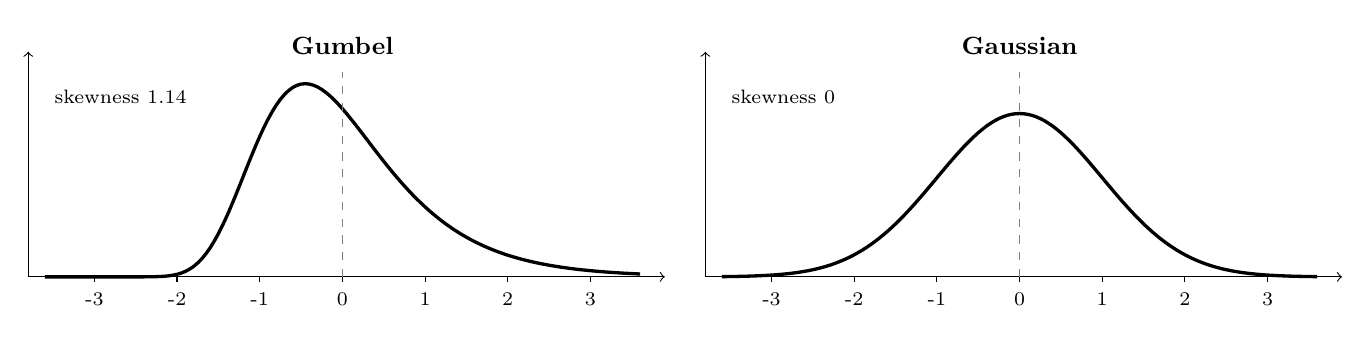
\begin{tikzpicture}[x=1.05cm,y=5.2cm]
  \begin{scope}
    \draw[->] (-3.8,0) -- (3.9,0);
    \draw[->] (-3.8,0) -- (-3.8,0.55);
    \foreach \x in {-3,-2,-1,0,1,2,3}
      {\draw (\x,0) -- (\x,-0.012); \node[font=\scriptsize,anchor=north] at (\x,-0.016) {\x};}
    \draw[very thick] plot coordinates {(-3.600,0.0000) (-3.550,0.0000) (-3.500,0.0000) (-3.450,0.0000) (-3.400,0.0000) (-3.350,0.0000) (-3.300,0.0000) (-3.250,0.0000) (-3.200,0.0000) (-3.150,0.0000) (-3.100,0.0000) (-3.050,0.0000) (-3.000,0.0000) (-2.950,0.0000) (-2.900,0.0000) (-2.850,0.0000) (-2.800,0.0000) (-2.750,0.0000) (-2.700,0.0000) (-2.650,0.0000) (-2.600,0.0000) (-2.550,0.0000) (-2.500,0.0000) (-2.450,0.0000) (-2.400,0.0001) (-2.350,0.0002) (-2.300,0.0003) (-2.250,0.0006) (-2.200,0.0010) (-2.150,0.0016) (-2.100,0.0026) (-2.050,0.0042) (-2.000,0.0063) (-1.950,0.0093) (-1.900,0.0134) (-1.850,0.0187) (-1.800,0.0255) (-1.750,0.0340) (-1.700,0.0443) (-1.650,0.0566) (-1.600,0.0709) (-1.550,0.0872) (-1.500,0.1055) (-1.450,0.1257) (-1.400,0.1474) (-1.350,0.1706) (-1.300,0.1948) (-1.250,0.2198) (-1.200,0.2452) (-1.150,0.2705) (-1.100,0.2955) (-1.050,0.3197) (-1.000,0.3429) (-0.950,0.3647) (-0.900,0.3849) (-0.850,0.4032) (-0.800,0.4195) (-0.750,0.4336) (-0.700,0.4455) (-0.650,0.4552) (-0.600,0.4626) (-0.550,0.4678) (-0.500,0.4708) (-0.450,0.4718) (-0.400,0.4709) (-0.350,0.4681) (-0.300,0.4637) (-0.250,0.4578) (-0.200,0.4505) (-0.150,0.4420) (-0.100,0.4324) (-0.050,0.4219) (0.000,0.4107) (0.050,0.3989) (0.100,0.3865) (0.150,0.3738) (0.200,0.3608) (0.250,0.3477) (0.300,0.3345) (0.350,0.3212) (0.400,0.3080) (0.450,0.2950) (0.500,0.2821) (0.550,0.2695) (0.600,0.2572) (0.650,0.2451) (0.700,0.2334) (0.750,0.2221) (0.800,0.2111) (0.850,0.2004) (0.900,0.1902) (0.950,0.1804) (1.000,0.1709) (1.050,0.1619) (1.100,0.1532) (1.150,0.1449) (1.200,0.1370) (1.250,0.1294) (1.300,0.1223) (1.350,0.1154) (1.400,0.1089) (1.450,0.1027) (1.500,0.0969) (1.550,0.0913) (1.600,0.0861) (1.650,0.0811) (1.700,0.0764) (1.750,0.0719) (1.800,0.0677) (1.850,0.0637) (1.900,0.0599) (1.950,0.0564) (2.000,0.0530) (2.050,0.0499) (2.100,0.0469) (2.150,0.0441) (2.200,0.0414) (2.250,0.0390) (2.300,0.0366) (2.350,0.0344) (2.400,0.0323) (2.450,0.0304) (2.500,0.0285) (2.550,0.0268) (2.600,0.0251) (2.650,0.0236) (2.700,0.0222) (2.750,0.0208) (2.800,0.0195) (2.850,0.0183) (2.900,0.0172) (2.950,0.0162) (3.000,0.0152) (3.050,0.0142) (3.100,0.0134) (3.150,0.0125) (3.200,0.0118) (3.250,0.0110) (3.300,0.0104) (3.350,0.0097) (3.400,0.0091) (3.450,0.0086) (3.500,0.0080) (3.550,0.0075) (3.600,0.0071)};
    \draw[dashed,gray] (0,0) -- (0,0.50);
    \node[font=\small\bfseries,anchor=south] at (0,0.52) {Gumbel};
    \node[font=\scriptsize,anchor=west] at (-3.6,0.44) {skewness $1.14$};
  \end{scope}
  \begin{scope}[xshift=8.6cm]
    \draw[->] (-3.8,0) -- (3.9,0);
    \draw[->] (-3.8,0) -- (-3.8,0.55);
    \foreach \x in {-3,-2,-1,0,1,2,3}
      {\draw (\x,0) -- (\x,-0.012); \node[font=\scriptsize,anchor=north] at (\x,-0.016) {\x};}
    \draw[very thick] plot coordinates {(-3.600,0.0006) (-3.550,0.0007) (-3.500,0.0009) (-3.450,0.0010) (-3.400,0.0012) (-3.350,0.0015) (-3.300,0.0017) (-3.250,0.0020) (-3.200,0.0024) (-3.150,0.0028) (-3.100,0.0033) (-3.050,0.0038) (-3.000,0.0044) (-2.950,0.0051) (-2.900,0.0060) (-2.850,0.0069) (-2.800,0.0079) (-2.750,0.0091) (-2.700,0.0104) (-2.650,0.0119) (-2.600,0.0136) (-2.550,0.0154) (-2.500,0.0175) (-2.450,0.0198) (-2.400,0.0224) (-2.350,0.0252) (-2.300,0.0283) (-2.250,0.0317) (-2.200,0.0355) (-2.150,0.0396) (-2.100,0.0440) (-2.050,0.0488) (-2.000,0.0540) (-1.950,0.0596) (-1.900,0.0656) (-1.850,0.0721) (-1.800,0.0790) (-1.750,0.0863) (-1.700,0.0940) (-1.650,0.1023) (-1.600,0.1109) (-1.550,0.1200) (-1.500,0.1295) (-1.450,0.1394) (-1.400,0.1497) (-1.350,0.1604) (-1.300,0.1714) (-1.250,0.1826) (-1.200,0.1942) (-1.150,0.2059) (-1.100,0.2179) (-1.050,0.2299) (-1.000,0.2420) (-0.950,0.2541) (-0.900,0.2661) (-0.850,0.2780) (-0.800,0.2897) (-0.750,0.3011) (-0.700,0.3123) (-0.650,0.3230) (-0.600,0.3332) (-0.550,0.3429) (-0.500,0.3521) (-0.450,0.3605) (-0.400,0.3683) (-0.350,0.3752) (-0.300,0.3814) (-0.250,0.3867) (-0.200,0.3910) (-0.150,0.3945) (-0.100,0.3970) (-0.050,0.3984) (0.000,0.3989) (0.050,0.3984) (0.100,0.3970) (0.150,0.3945) (0.200,0.3910) (0.250,0.3867) (0.300,0.3814) (0.350,0.3752) (0.400,0.3683) (0.450,0.3605) (0.500,0.3521) (0.550,0.3429) (0.600,0.3332) (0.650,0.3230) (0.700,0.3123) (0.750,0.3011) (0.800,0.2897) (0.850,0.2780) (0.900,0.2661) (0.950,0.2541) (1.000,0.2420) (1.050,0.2299) (1.100,0.2179) (1.150,0.2059) (1.200,0.1942) (1.250,0.1826) (1.300,0.1714) (1.350,0.1604) (1.400,0.1497) (1.450,0.1394) (1.500,0.1295) (1.550,0.1200) (1.600,0.1109) (1.650,0.1023) (1.700,0.0940) (1.750,0.0863) (1.800,0.0790) (1.850,0.0721) (1.900,0.0656) (1.950,0.0596) (2.000,0.0540) (2.050,0.0488) (2.100,0.0440) (2.150,0.0396) (2.200,0.0355) (2.250,0.0317) (2.300,0.0283) (2.350,0.0252) (2.400,0.0224) (2.450,0.0198) (2.500,0.0175) (2.550,0.0154) (2.600,0.0136) (2.650,0.0119) (2.700,0.0104) (2.750,0.0091) (2.800,0.0079) (2.850,0.0069) (2.900,0.0060) (2.950,0.0051) (3.000,0.0044) (3.050,0.0038) (3.100,0.0033) (3.150,0.0028) (3.200,0.0024) (3.250,0.0020) (3.300,0.0017) (3.350,0.0015) (3.400,0.0012) (3.450,0.0010) (3.500,0.0009) (3.550,0.0007) (3.600,0.0006)};
    \draw[dashed,gray] (0,0) -- (0,0.50);
    \node[font=\small\bfseries,anchor=south] at (0,0.52) {Gaussian};
    \node[font=\scriptsize,anchor=west] at (-3.6,0.44) {skewness $0$};
  \end{scope}
\end{tikzpicture}
\caption{The two noise laws, each standardized to mean zero and variance one, so that only
shape distinguishes them. Give every alternative a location, add a draw from the left-hand
density to each, and take the highest: the winning probabilities are Equation~\eqref{eq:luce},
and restricting the field renormalizes the shares proportionally. Do the same with the
right-hand density and the shares contract instead. Renormalization is therefore a race too,
run with a noise law that is asymmetric and long-tailed to the right. We
withhold our opinion as to which is the more \emph{a priori} reasonable.}
\label{fig:noise}
\end{figure}

The two laws compared here sit at opposite ends of the concavity condition. The Gaussian
satisfies it strictly, since
$\frac{d^2}{dx^2}\log r(x) = -\operatorname{Var}(Z \mid Z < x) < 0$. The Gumbel has
$r(x) = s^{-1}e^{-x/s}$, so $\log r$ is affine, the inequality becomes an equality, and
renormalization is recovered exactly, which is the Holman--Marley construction
\cite{lucesuppes1965,holman1974}. The axiom is a boundary of the class, and it is where
machine learning sits: a softmax over scores $z_i$ is Equation~\eqref{eq:luce} with
$u(i) = \exp(z_i)$, so masking a softmax and rescaling the survivors is proportional
renormalization.

A deep network is not committed to the axiom. Its logits are the output of
an arbitrarily flexible function, and it can represent any distribution over its full
vocabulary, including distributions that no independent additive random-utility model
generates. All of that is true, and none of it touches the case at hand. The constraint applies
to a \emph{fixed} logit vector at inference time. Depth governs the map from context to logits;
it says nothing about how the distribution should change when the support is cut and the logits
are not recomputed. Masking and rescaling a fixed vector leaves every surviving ratio exactly as
it was, which is Equation~\eqref{eq:luce} on the restricted set, however that vector was
produced and however deep the network that produced it.

Escaping the axiom therefore requires recomputing the scores with the permitted set as part of
the input. A model trained that way can express any dependence on the menu, and its masked
distribution is then not a transport of its unmasked one, so the question this paper asks does
not arise for it. The question arises where a score vector is computed once and then restricted
\emph{and} the restriction is an intervention on what may be chosen rather than news about a
fixed experiment. Constrained decoding, vocabulary masking, restricted action spaces and post-hoc
class removal are all candidates, but which of them qualifies depends on the intended estimand
and not on the code. Where the target is the conditional law of the unrestricted model, masking is
correct and nothing here applies.

The proposition gives the direction of the effect and not its size. Size depends on the shares
as well as on the noise law, and recalibrating several laws to one share vector and then to
another can reverse which of them contracts more, so tail thickness alone does not order the
laws by how much they contract.

\subsection{Gaussian taste heterogeneity as a mechanism}
\label{sec:mixture}

Nothing so far explains why the Gaussian member of the class should be the one that fits.
We provide a plausibility argument applying only to aggregate shares.

Let every individual obey the axiom, and let their tastes differ. Individual $\theta$
assigns systematic utility $V_i(\theta)$ to alternative $i$ and chooses by Luce at scale
$\beta > 0$,
\begin{equation}
P_S(i \mid \theta) = \frac{\exp\{V_i(\theta)/\beta\}}{\sum_{j \in S}\exp\{V_j(\theta)/\beta\}},
\label{eq:condluce}
\end{equation}
which by Yellott's theorem is the same as choosing the largest
$V_i(\theta) + \beta G_i(\theta)$ for independent standard Gumbel $G_i(\theta)$.

\begin{proposition}[Gaussian taste heterogeneity]
\label{prop:mixture}
Suppose $V_i(\theta) = \mu_i + \sigma Z_i(\theta)$ with $Z(\theta) \sim N(0,I_K)$
independently across individuals. Then the aggregate choice probabilities are exactly the
winning probabilities of a contest with utilities
\begin{equation}
\mu_i + \sigma Z_i + \beta G_i ,
\label{eq:composite}
\end{equation}
independent across alternatives. If $\mu_i = \sigma a_i$ and $\sigma/\beta \to \infty$, they
converge to those of Case V with locations $a$.
\end{proposition}

\begin{proof}
Aggregating over individuals integrates over the taste draw $Z$, leaving the
per-alternative utility \eqref{eq:composite}, independent across $i$ because both
components are. Dividing every utility by $\sigma$ preserves the $\arg\max$ and gives
$a_i + Z_i + (\beta/\sigma)G_i$, whose last term vanishes in probability. Ties have
probability zero under the Gaussian limit, so the winning probabilities converge.
\end{proof}

This is a mixed logit: Gaussian heterogeneity between individuals, Gumbel noise within
them. Such models are standard, and McFadden and Train \cite{mcfaddentrain2000} establish
how general they are. The proposition adds only the link between the high-heterogeneity limit of
that familiar object and the restriction map tested here.

The Gaussian assumption on taste can itself be derived from a limit theorem.

\begin{corollary}[Many small taste components]
\label{cor:clt}
Suppose $V_i(\theta) = \sqrt{m}\,a_i + \sum_{\ell=1}^{m}\xi_{\ell i}(\theta)$, where the
vectors $\xi_\ell(\theta)$ are independent and identically distributed across $\ell$ with mean
zero, covariance $I_K$ and finite second moments, and the individual chooses by \eqref{eq:condluce} at fixed
$\beta$. Then the aggregate choice probabilities converge as $m \to \infty$ to those of
Case V with locations $a$.
\end{corollary}

\begin{proof}
Dividing the utilities by $\sqrt{m}$ gives
$a_i + m^{-1/2}\sum_\ell \xi_{\ell i} + (\beta/\sqrt{m})G_i$. The multivariate central limit
theorem sends the middle term to $N(0,I_K)$ and the last to zero, and the $\arg\max$
probabilities are continuous at a limit with no ties.
\end{proof}

A correction to this limit must be a correction to shape, not to scale. For any
location-scale family $X_i = a_i + s\varepsilon_i$ the winning probabilities satisfy
$P^S_i(a;s) = P^S_i(a/s;1)$, so if $b(p)$ is the unit-scale location vector calibrated to the
full-menu shares $p$, then $s\,b(p)$ is the scale-$s$ calibration and
$P^T_i(s\,b(p);s) = P^T_i(b(p);1)$ for every restricted menu $T$. A common noise scale is
therefore a gauge: it is absorbed exactly by the fitted locations, not approximately, and restricted-menu
observations cannot identify it either unless the locations are anchored by cardinal
information from outside the shares.

The same holds for the composite noise $W_\varepsilon = Z + \varepsilon G$ at finite
$\sigma/\beta$, with $\varepsilon = \beta/\sigma$. Subtract the common Gumbel mean, which
cancels in the $\arg\max$, and divide by $s_\varepsilon = (1 + \varepsilon^2 \pi^2/6)^{1/2}$,
which is a gauge by the previous paragraph. The standardized law then has skewness of order
$\varepsilon^3$ and excess kurtosis of order $\varepsilon^4$, with no $\varepsilon^2$ term
surviving. Under smooth dependence of the winning probabilities on the noise law, and a
locally nonsingular Jacobian of the full-menu share map in the $K-1$ location contrasts, the
implicit function theorem gives $a_\varepsilon(p) = a_0(p) + O(\varepsilon^3)$, so the first
generic departure of the recalibrated restriction map from Case V is cubic in $\varepsilon$.
Symmetric configurations can cancel the cubic term and leave a higher order.

Any parameter that interpolates between the two maps has to be a shape or relative-mixture
parameter. It cannot be a common noise scale.

The covariance assumption is not innocuous. If the taste
components carry covariance $\Sigma$ instead of $I_K$, the same argument delivers a Gaussian
race with covariance $\Sigma$, which is correlated multinomial probit rather than Case V.
Case V additionally requires the covariance to be isotropic on the $(K-1)$-dimensional
utility-contrast subspace. In the usual reference-difference coordinates
$D_i = \varepsilon_i - \varepsilon_K$ that is not a diagonal matrix: independent equal-variance
errors give $\operatorname{Cov}(D) = \sigma^2(I_{K-1} + \mathbf{1}\mathbf{1}^{\top})$, and it is
in an orthonormal contrast basis $Q$ that $Q^{\top}\operatorname{Cov}(\varepsilon)Q =
\sigma^2 I_{K-1}$. So the limit
theorem motivates Gaussian random utility in general, and independence across alternatives
is a further restriction, adopted here because it is the parameter-free member of the class.

\begin{table}[ht]
\centering
\small
\begin{tabular}{rrrrr}
\toprule
$\sigma$ & Top share & Observed $\lambda$ & Case V $\lambda$ & Ratio \\
\midrule
$0.5$ & $0.255$ & $0.052$ & $0.225$ & $0.23$ \\
$1$ & $0.300$ & $0.128$ & $0.227$ & $0.57$ \\
$2$ & $0.343$ & $0.197$ & $0.229$ & $0.86$ \\
$3$ & $0.359$ & $0.216$ & $0.229$ & $0.94$ \\
$4$ & $0.365$ & $0.228$ & $0.230$ & $0.99$ \\
$6$ & $0.372$ & $0.225$ & $0.230$ & $0.98$ \\
$8$ & $0.373$ & $0.230$ & $0.231$ & $1.00$ \\
$16$ & $0.375$ & $0.233$ & $0.231$ & $1.01$ \\
\bottomrule
\end{tabular}
\caption{A population of Luce choosers whose log-worths carry Gaussian taste variation of
scale $\sigma$ against a Gumbel choice-noise scale of $1$, with locations scaled as
$\sigma a$ so that the shares do not degenerate. The contraction slope $\lambda$ is defined on
pairs by $\delta_{ij} = \operatorname{logit} q_{ij} - \log(p_i/p_j)$ for $i$ the
higher-share alternative, with $q_{ij}$ the observed share preferring $i$ from
$\{i,j\}$, fitted through the origin as $\delta = -\lambda \log(p_i/p_j)$; $\lambda = 0$ is
exact renormalization. Observed $\lambda$ is the population's
contraction; Case V $\lambda$ is what the independent unit-variance Gaussian contest implies
for that population's own shares. The top share is reported to show the limit is not the
near-indifference corner. Parameters: $K = 5$, $A = (0.55, 0.25, 0, -0.25, -0.55)$ with
$\mu = \sigma A$, Gumbel scale $1$, and $400{,}000$ direct Monte Carlo draws per row from
\texttt{numpy.random.default\_rng(0)}; reproduced by
\texttt{python heterogeneity\_limit.py}.}
\label{tab:mixture}
\end{table}

No individual need be non-Lucean for the aggregate to approach the Gaussian transport. A
population of Luce choosers whose tastes vary is a contest with composite noise, and as taste
variation comes to outweigh within-person choice noise the composite approaches Gaussian and the
population contraction approaches the Case V prediction. At any finite ratio the exact law is
Gaussian plus Gumbel, not Gaussian, so Case V is the limit and not the aggregate itself.
That mechanism also says where the fit should be worst: in populations whose members are
nearly alike. It explains movement from linear renormalization toward Case V and no further.
The composite path approaches $r = 1$ from below, so it does not account for the median $r$ of
$1.16$ in Figure~\ref{fig:line}, nor for the fifteen of twenty populations that contract past
Case V. That residual is unexplained here. Dependence, non-isotropic heterogeneity, menu-dependent
attention and some third standardized shape are all candidates.

Independent evidence for the same phenomenon exists in memory research. Robinson, DeStefano,
Vul and Brady \cite{robinson2023} put softmax against Gaussian signal detection across
$m$-alternative recognition tasks, and report that ``the $d'$ parameter of the Gaussian signal
detection model was more stable across $m$-afc conditions than the $\beta$ parameter of the
softmax model''. Their primary analysis holds each model's parameter fixed across all $m$
conditions and compares log likelihood, and the Gaussian wins in both experiments,
$t(29) = 4.26$ and $t(29) = 4.42$, $p < .001$, with thirty participants each. That is the
contraction studied here, showing up as a parameter that has to move with the size of the menu.

Their design is the nearest to this one that we have found. Three differences remain. No response
set is restricted over shared alternatives:
$m$ varies by adding fresh items, not by withdrawing named ones. Linear renormalization is
never the competitor, since the comparison is softmax against Gaussian with both fitted. And the
parameters are estimated on the data that scores them, so the cross-condition constraint does the
work that holding out a menu does here. What their result establishes is that one parameter has
to move with $m$ and the other does not, which shows contraction is present without measuring
how large it is.

\subsection{Correlated probit and the unidentified covariances}
\label{sec:probit}

Correlated multinomial probit can represent near-substitution, by giving two similar
alternatives a positive covariance. It does not follow that it represents any near-substitute
behaviour exactly: menu-dependent attention and the dimensional retuning of
Section~\ref{sec:boundary} are not captured by a static covariance. And it is not available as a
default.

One full-menu share vector supplies $K-1$ free numbers, and those are already exhausted by the $K-1$ location
contrasts. After choosing a reference alternative and normalizing scale, the covariance matrix
of the $K-1$ utility differences carries a further $K(K-1)/2 - 1$ parameters. A single
$(K-1)$-dimensional share vector cannot jointly identify $K-1$ location contrasts and an
unrestricted covariance shape, so for every $K \ge 3$ the covariance is unidentified from
full-menu shares alone. A correlated model is available to anyone with
restricted-menu data to fit it on. That is a different exercise from the one conducted here.

\section{Empirical}
\label{sec:empirical}

\subsection{Protocol}
\label{sec:design}

Both maps are calibrated on full-menu shares alone, then scored by log
loss on restricted menus neither has seen. The input is a probability vector and nothing else,
which is what makes the two maps comparable and what the exercise assumes.

Both maps hold the latent quantity fixed and change only the menu, and
Section~\ref{sec:boundary} collects the cases where that fails. Two further assumptions are less
visible. The noise is independent and identically shaped across alternatives, which
near-substitutes violate. And the population is treated as one chooser with one latent vector,
though Section~\ref{sec:mixture} shows heterogeneous Luce choosers reproducing aggregate
contraction with no individual departing from the axiom.

Three developments make the comparison possible now. Trial-level archives are open, so restricted menus can be
scored on the observations that produced them rather than on printed marginals. Inverting
Equation~\eqref{eq:winprob} from shares alone is a single pass over a shared grid, so the
Gaussian map costs nothing to apply. And a generative null is available.

Contraction of a noisily
estimated share vector lowers log loss whether or not the axiom fails, so every raw gain below is
accompanied by the gain a population obeying the axiom exactly would produce on the same menus,
its centred excess, and a null frequency. The excess is a diagnostic centred on that particular
fitted null, not an estimate of a model-free structural effect: under a non-Luce population there
is no reason for the null's bias to match the alternative's. Section~\ref{sec:null} details the
construction.

\subsection{Restrictions that were observed}
\label{sec:observed}

Ten collections record choices from a smaller menu directly, and they are reported first because
nothing about the restriction is inferred. The first three are controlled: the same subjects, or
the same stimuli, before and after a menu change. The remainder are ecological, and
Section~\ref{sec:more} says where that weakens them.

\subsubsection{Consumer goods, all subsets of five}
\label{sec:menus}

In the ranking-and-menu benchmark of Tables~\ref{tab:menus} and~\ref{tab:heldout}, twelve
collections are complete rankings from which subset choice is read off, and one observes menu
choice directly. That one comes first.

Costa-Gomes, Cueva, Gerasimou and Teji\v{s}\v{c}\'ak \cite{costagomes2022} ran two
experiments in which subjects chose separately from every non-singleton subset of five
consumer goods, twenty-six menus; the first also included the five singletons. The archive
names the goods by two-letter codes and we describe them no more precisely. Restriction is
observed rather than imputed, which makes this the cleanest test in our collection, and the
two experiments are separate studies with disjoint subjects, so we report them separately
rather than pooled.

Subjects are split into five folds. On the training subjects, shares come only from the full
five-item menu; both maps are calibrated to those shares and nothing else; each then predicts
every menu of size two, three and four; and we score the choices actually made by held-out
subjects. Intervals resample subjects and repeat the whole procedure, calibration included.
Subjects who may defer are reported alongside the forced-choice subgroup, for whom no
deferral coding enters. Of the $373$ subjects, $364$ record at least one usable choice from a
non-singleton menu and enter the analysis.

\begin{table}[ht]
\centering
\small
\begin{tabular}{lrrrrrr}
\toprule
& $n$ & Choices & Linear & Gaussian & Gain & Excess \\
\midrule
Experiment 1, all & 230 & 5{,}134 & $0.9438$ & $0.9298$ & $+0.0140$ & $+0.0158$ \\
Experiment 1, forced & 76 & 1{,}900 & $0.9639$ & $0.9197$ & $+0.0442$ & $+0.0466$ \\
Experiment 2, all & 134 & 3{,}105 & $0.9162$ & $0.9103$ & $+0.0059$ & $+0.0056$ \\
Experiment 2, forced & 61 & 1{,}525 & $0.8939$ & $0.8799$ & $+0.0140$ & $+0.0131$ \\
\midrule
Pooled & 364 & 8{,}239 & $0.9263$ & $0.9164$ & $+0.0100$ & $+0.0123$ \\
\bottomrule
\end{tabular}
\caption{Held-out log loss per choice on menus of size two to four, both maps calibrated only
to training-fold full-menu shares under a common add-$\alpha$ convention, $\alpha = 1/2$.
Excess is the gain net of the median gain under a population that renormalizes exactly, as in
Section~\ref{sec:null}. Subject-bootstrap intervals for the gains are
$[+0.0072, +0.0335]$, $[+0.0171, +0.0867]$, $[+0.0009, +0.0306]$, $[+0.0034, +0.0560]$ and
$[+0.0048, +0.0246]$ respectively.}
\label{tab:menus}
\end{table}

Gaussian renormalization is ahead in both experiments and in both treatments, and by more where deferral
cannot interfere. The two experiments do not agree on strength. Experiment 1 clears its null
comfortably, with null frequencies of $0.010$ and $0.005$; experiment 2, at
fifty-eight per cent of the sample, does not, at $0.199$ and $0.129$. The direction
replicates and the magnitude is not established by these data alone.

\subsubsection{Colours and symbols, with the menu revealed after the stimulus}
\label{sec:after}

In the consumer experiment the subject sees the reduced menu before deciding, so preferences
could in principle be formed with the restriction already known. The two perceptual experiments
below do not allow that.

Yeon and Rahnev \cite{yeonrahnev2020} show a display whose dominant colour, among four, has
to be named. In one condition the full menu is available. In a second the observer sees the
identical display and is told only \emph{after} it has gone which two named alternatives the
answer lies between. The two conditions were run in separate blocks of trials, so the observer
knew which condition they were in and had practised it. What they could not know, while looking
at the display, was which two colours the pair would turn out to be. They could not attend
selectively to those two colours in advance, though they did know that only two would be
offered. Their Experiment 2 repeats this with six symbols.

Calibration uses that observer's full-menu row for that dominant item alone, and the
two-alternative cells on the same observer and item are then predicted and scored.

\begin{table}[ht]
\centering
\small
\begin{tabular}{lrrrrr}
\toprule
Arm & Cells & Linear & Gaussian & Gain & Excess \\
\midrule
Four colours, menu revealed after & 384 & $0.4942$ & $0.4795$ & $+0.0147$ & $+0.0157$ \\
Six symbols, menu revealed after & 300 & $0.6276$ & $0.5999$ & $+0.0278$ & $+0.0314$ \\
\midrule
Same pairs, announced in advance & 384 & $0.3967$ & $0.3928$ & $+0.0038$ & $+0.0048$ \\
\bottomrule
\end{tabular}
\caption{Mean nats per cell, a cell being one observer, one dominant item and one surviving
alternative. Subject-bootstrap intervals for the gains are $[+0.0118, +0.0179]$,
$[+0.0234, +0.0324]$ and $[+0.0006, +0.0072]$. The null here resamples the calibration row
as well as the pair counts, so it charges Gaussian renormalization for calibration noise as well as for
sampling noise in what it predicts; all three null frequencies are at the $0.005$ floor.}
\label{tab:after}
\end{table}

The six-symbol gain is the larger of the two arms. The same pairs were also run \emph{announced in advance}, so the
observer can aim attention at them. That arm was not analysed by the original authors and is
recovered here from the trial files. There the advantage nearly disappears. Accuracy rises from $0.780$
to $0.850$, linear renormalization becomes almost exactly right, and Gaussian renormalization begins to
over-contract.

So the advantage is not a property of these pairs, these colours or
these observers. It appears when the surviving pair is selected only after the percept has formed, so that
attention cannot be tailored to that pair, and it does not appear when the pair is named in
advance.

In both genuine restriction arms \emph{both} maps over-predict the favourite: linear renormalization by $0.069$ and Gaussian renormalization by
$0.055$ at four alternatives, and by $0.096$ and $0.064$ at six. Contraction has the right
sign and removes a fifth to a third of the error. Neither of the two maps is calibrated
here, and a fitted shape or mixture parameter has room to improve on both. That over-prediction is Yeon and
Rahnev's own finding, reached with a fitted model, so their result is independent evidence
that the correction runs toward contraction while bounding what either default can claim.

Utochkin, Azarov and Grigorev \cite{utochkin2025} supply the same structure in memory. An
observer sees a studied photograph among three foils, or the same target against one named
foil, with the same images in both arms. Gaussian renormalization wins by $+0.0037$ per cell over $360$
nested cells, interval $[+0.0029, +0.0047]$, the tightest in the paper. The contraction is
the same size against a foil from the target's own category as against a foil from another,
which matters in Section~\ref{sec:boundary}: category membership is not what breaks
independence.

\subsubsection{Gambles, ballots, news slates and Wikipedia links}
\label{sec:more}

Restriction is observed in four further populations, which differ in what does the removing.

A fifth candidate was tried and discarded. Grocery stockout data records hourly sales by
product,
and a shopper may buy two items from one category, so the alternatives are not mutually
exclusive and the object is a basket rather than a choice. Recovering choices would need
transaction-level baskets, which the release does not contain.

Aguiar, Boccardi, Kashaev and Kim \cite{aguiar2023} observe choices from all thirty-one
non-empty subsets of five lotteries with a default always available, so menus run from two
to six alternatives, in a cross-section giving at most two disjoint menus per person. It is adversarial on the authors' own
analysis, since they report that random utility cannot explain the population behaviour
while a logit attention model survives.

The experiment was run three times on disjoint subject pools, differing only in how much
arithmetic is needed to value an alternative: one operation, three, or five. The excess
over the null rises with that requirement, from $-0.0012$ to $+0.0045$ to $+0.0081$, and
the full-menu shares flatten alongside it, the largest falling from $0.357$ to $0.257$
against a six-alternative maximum entropy of $1.792$.

We read the gradient as consistent with the mechanism rather than as instability, though
increased random responding, attention failure or a change in what subjects consider would
produce the same ordering. When the arithmetic is one
step the task has a computable answer and is closer to an examination question than to a
preference judgement; subjects converge, the shares concentrate, and there is little
preference left for any restriction map to describe. When it takes five steps nobody can
compute the answer, so people fall back on what they actually prefer and the choice becomes
psychological. A model of preference under noise should win in the second case and not the
first. Winning in both, including where the answer is objectively determined, would be the
result to distrust.

US presidential ballots supply restriction by statute. The alternatives are the same named
candidates in every state and which of them appears varies with petition thresholds and
filing deadlines, so the states are nested menus over identical alternatives. States are
not interchangeable populations, so a state may only predict another whose two-party log
odds are within $0.5$.

News slates supply the largest sample and the only menus that are recorded rather than
reconstructed. The Microsoft News dataset logs, for each impression, the exact set of
articles displayed and which one was clicked \cite{wu2020}. Slates recur across users and
one slate is frequently a subset of another, so click shares on the larger slate calibrate
both maps and the choices made on the nested smaller one score them. Of $153{,}727$
impressions, $846$ slates recur ten or more times and yield $6{,}135$ nested pairs, of which the first
$6{,}000$ are scored. Because
those pairs are drawn from a few hundred slates and overlap heavily, the interval below
resamples slates rather than pairs.

Wikipedia links supply editorial removal, in the weakest form of observation used here. The
clickstream release is not a record of impressions: it is a monthly count of (referrer, resource)
transitions extracted from request logs, so what it supplies is the aggregate distribution of
destinations conditional on a transition having been made from a given article, and not a table
with one row per reader carrying a menu and one exclusive response. Destinations are the same
articles from month to month and editors change the set, so adjacent dumps give the earlier
month's conditional shares and the later month's. The dump censors pairs below ten clicks, so a
vanished destination may have been removed or may have fallen below threshold; it records no link
position, so layout is uncontrolled; and readership and page content move between months along
with the link set. This row is a transport comparison on conditional transition shares rather
than an observed withdrawal.

\begin{table}[ht]
\centering
\small
\begin{tabular}{lrrrrr}
\toprule
Population & Units & Gain & Null median & Excess & Null freq. \\
\midrule
Lotteries, high cost & 3{,}928 & $+0.0101$ & $+0.0020$ & $+0.0081$ & $.035$ \\
Lotteries, medium cost & 3{,}928 & $+0.0068$ & $+0.0023$ & $+0.0045$ & $.124$ \\
Lotteries, low cost & 3{,}928 & $+0.0002$ & $+0.0014$ & $-0.0012$ & $.667$ \\
News slates & 6{,}000 pairs & $+0.0496$ & $-0.0088$ & $+0.0584$ & $.016$ \\
US state ballots 2024 & 263 pairs & $+0.0002$ & $-0.0000$ & $+0.0002$ & $.005$ \\
Wikipedia links & 3{,}544 pages & $-0.0001$ & $-0.0002$ & $+0.0001$ & $.005$ \\
\bottomrule
\end{tabular}
\caption{Held-out loss differences on populations where restriction is observed rather
than read off a ranking. Excess is the gain net of what a renormalizing population
produces on the same menus. The lottery frames are disjoint subject pools; ballot units
are matched state pairs; Wikipedia units are pages whose destination set shrank; One row, Wikipedia, has a
negative raw gain and a positive excess, which means Gaussian renormalization loses in absolute
terms while still departing from the axiom in the direction of contraction.}
\label{tab:more}
\end{table}

The news result is the largest in this table, about five times the next, on the only menus in the paper
that were recorded at the moment of choice. Its weakness is assignment: the slates are chosen
by a recommender, so a slate's composition is correlated with what the system expects readers
to want, and a smaller slate may reach a different readership than the larger one. Both maps
inherit that identically and the null runs on the same slates. That does not make the
comparison clean. The null holds the worths fixed and so does not simulate a shift in
readership, position or context, and two maps facing the same confound need not respond to it
equally well. This row and the two below it are transport exercises on data that was not
generated by withdrawing an alternative from a fixed population, and they are weaker evidence
about withdrawal than the controlled restrictions of Sections~\ref{sec:menus}
and~\ref{sec:after} for that reason.

The lottery gradient runs with arithmetic cost, and the mechanism of
Section~\ref{sec:mixture} predicts its direction, since computation error is per-alternative and
roughly Gaussian, so loading more of it onto each alternative raises $\sigma$ against $\beta$.

On the Wikipedia rows, tightening the filter that identifies a genuine removal from a five per
cent share to thirty-five per cent raises the excess from $+0.0001$ to $+0.0005$ across
$3{,}544$, $817$ and $121$ pages. That is consistent with attenuation by measurement, and also
with the threshold selecting a different population of pages, which these data cannot separate.

Wikipedia and the two General Social Survey collections put the
truth between the two maps, contracting when an alternative goes but by less than Case V says.
They are the exception. Fitting the contraction slope $\lambda$ of Table~\ref{tab:mixture} to
each collection's observed pairwise choices puts the observed slope \emph{above} Case V's in
eight of eleven, so in most collections choice contracts by more than Case V predicts and
Gaussian renormalization errs by over-predicting the favourite. That is the same direction as
the after-stimulus arms of Section~\ref{sec:after}, where both maps over-predict, and it says
the Gaussian point of the family is not far enough along it for these populations.




\subsection{Restrictions induced from rankings}
\label{sec:rankings}

Twelve archival collections have human respondents and rankings, or ratings fine enough
to yield them. Two rank-order card tasks from the General Social Survey ask what a
child should learn and what matters in a job. Three independent samples of Jester users
rate the same ten jokes. Sushi rankings come from a Japanese web survey, film rankings
are induced from Netflix ratings, and dots and puzzles are perceptual discrimination
tasks. The rest are rankings of seven sports by participation preference, ten
occupations by perceived prestige, and four political goals from a five-nation survey.

The thirteen collections comprise $147{,}719$ responses, of which the menu experiment
contributes $373$ subjects; the twelve ranking collections contribute $147{,}346$.
These are not thirteen independent experiments, since three are Jester files, two are
General Social Survey items, and dots and puzzles are companion tasks.

The protocol matches Section~\ref{sec:menus} with respondents in place of subjects, and
the outcome for a subset is the respondent's highest-ranked member of it.

\begin{table}[ht]
\centering
\small
\begin{tabular}{lrrrrrl}
\toprule
Dataset & $n$ & $K$ & Subsets & Linear & Gaussian & Gain \\
\midrule
Occupational prestige & 143 & 10 & 1{,}012 & $1.0170$ & $0.9780$ & $+0.0391$ $[+0.0207, +0.0802]$ \\
Sushi & 5{,}000 & 10 & 1{,}012 & $1.3719$ & $1.3607$ & $+0.0111$ $[+0.0079, +0.0141]$ \\
Political goals & 2{,}262 & 4 & 10 & $0.8431$ & $0.8355$ & $+0.0076$ $[+0.0060, +0.0095]$ \\
GSS socialization & 5{,}000 & 5 & 25 & $0.7786$ & $0.7728$ & $+0.0057$ $[+0.0023, +0.0105]$ \\
Jester file 3 & 5{,}000 & 10 & 1{,}012 & $1.5182$ & $1.5158$ & $+0.0024$ $[+0.0014, +0.0031]$ \\
Jester file 1 & 5{,}000 & 10 & 1{,}012 & $1.5280$ & $1.5260$ & $+0.0020$ $[+0.0009, +0.0030]$ \\
Jester file 2 & 5{,}000 & 10 & 1{,}012 & $1.5240$ & $1.5223$ & $+0.0018$ $[+0.0012, +0.0031]$ \\
GSS job values & 5{,}000 & 5 & 25 & $0.8407$ & $0.8389$ & $+0.0018$ $[+0.0014, +0.0045]$ \\
Dots & 3{,}183 & 4 & 10 & $0.7862$ & $0.7845$ & $+0.0016$ $[+0.0007, +0.0026]$ \\
Netflix & 4{,}379 & 3 & 3 & $0.6961$ & $0.6949$ & $+0.0013$ $[+0.0008, +0.0016]$ \\
Puzzles & 3{,}180 & 4 & 10 & $0.7769$ & $0.7761$ & $+0.0008$ $[+0.0002, +0.0017]$ \\
\midrule
Sports participation & 130 & 7 & 119 & $1.2519$ & $1.2468$ & $+0.0051$ $[+0.0027, +0.0159]$ \\
\bottomrule
\end{tabular}
\caption{Held-out log loss per prediction over every proper restriction, $2 \le |T| < K$.
Datasets are capped at five thousand respondents for runtime. Gaussian renormalization is lower
in twelve of twelve and the interval excludes zero in all twelve. Occupational prestige is
scorable here only because the shared smoothing removes a zero training cell. Sports
participation sits below the rule: its gain is real but Section~\ref{sec:null} shows it
carries no evidence about the restriction map. Intervals resample respondents and refit the whole pipeline inside every
replicate, calibration and both maps and all subsets, so they carry calibration uncertainty;
one hundred replicates, or two hundred for the two collections under a thousand respondents.
Every interval excludes zero, including puzzles, whose earlier interval held the fitted models
fixed and covered it. Refitting widens most intervals and roughly trebles the width on GSS
socialization.}
\label{tab:heldout}
\end{table}

\subsection{Two conventions, and what they change}
\label{sec:conventions}

Neither map fits anything, but the pipeline around them makes two choices. Shares are smoothed
by add-$\alpha$ with $\alpha = 1/2$, and the aggregate weights every subset of size two or more
equally. Both are conventions rather than results, so both are varied.

\begin{table}[ht]
\centering
\small
\begin{tabular}{lrrrcrrr}
\toprule
& \multicolumn{3}{c}{smoothing} & & \multicolumn{3}{c}{menu weighting} \\
\cmidrule(r){2-4}\cmidrule(l){6-8}
Collection & $\alpha=0$ & $\alpha=\tfrac12$ & $\alpha=1$ & & subsets & by size & pairs \\
\midrule
Occupational prestige & n/a & $+.0391$ & $+.0153$ & & $+.0391$ & $+.0299$ & $+.0286$ \\
Sushi & $+.0113$ & $+.0111$ & $+.0109$ & & $+.0111$ & $+.0121$ & $+.0412$ \\
Political goals & $+.0076$ & $+.0076$ & $+.0076$ & & $+.0076$ & $+.0075$ & $+.0079$ \\
GSS socialization & $+.0060$ & $+.0057$ & $+.0055$ & & $+.0057$ & $+.0048$ & $+.0130$ \\
Sports participation & $+.0056$ & $+.0051$ & $+.0046$ & & $+.0051$ & $+.0045$ & $+.0058$ \\
Jester file 3 & $+.0024$ & $+.0024$ & $+.0024$ & & $+.0024$ & $+.0024$ & $+.0064$ \\
Jester file 1 & $+.0020$ & $+.0020$ & $+.0019$ & & $+.0020$ & $+.0019$ & $+.0053$ \\
Jester file 2 & $+.0018$ & $+.0018$ & $+.0017$ & & $+.0018$ & $+.0017$ & $+.0048$ \\
GSS job values & $+.0019$ & $+.0018$ & $+.0018$ & & $+.0018$ & $+.0017$ & $+.0021$ \\
Dots & $+.0017$ & $+.0016$ & $+.0016$ & & $+.0016$ & $+.0014$ & $+.0025$ \\
Netflix & $+.0013$ & $+.0013$ & $+.0013$ & & $+.0013$ & $+.0013$ & $+.0013$ \\
Puzzles & $+.0008$ & $+.0008$ & $+.0008$ & & $+.0008$ & $+.0007$ & $+.0013$ \\
\bottomrule
\end{tabular}
\caption{Held-out gain under three smoothing conventions and three menu weightings. Smoothing is
close to inert: eleven collections move by less than $0.0004$ across the three values.
Occupational prestige is the exception, unscorable at $\alpha = 0$ because a training cell is
empty and falling to $+0.0153$ at $\alpha = 1$, which is the collection with $143$ respondents and
ten alternatives. Weighting changes magnitude and not sign. Uniform by surviving size is smaller
throughout, pairs alone are larger, and Sushi runs from $+0.0108$ to $+0.0412$ depending which is
chosen. All thirty-six cells that can be computed are positive.}
\label{tab:conventions}
\end{table}

The weighting result matters for how the headline should be read. Every subset of size two or
more counting once puts most of the weight near $|T| = K/2$, and pairs are where the two maps
differ most, so the aggregate reported throughout is the conservative choice of the three rather
than a neutral one. The direction does not depend on it.

\subsection{What the score averages over}
\label{sec:estimand}

Three features of the score are choices rather than results, and each is varied here.

The first is which menus are scored. The estimand throughout is proper restrictions,
$2 \le |T| < K$. The full menu is excluded because it is not a restriction: both maps are
calibrated on those shares and both return them, so it contributes an identical zero. Its weight
is one subset in $2^K - K - 1$, which is one in $1{,}013$ at $K = 10$ and one in four at $K = 3$.
Including it would therefore shrink small collections and leave large ones alone, which is not a
conservative choice but a different and $K$-dependent estimand, and it would distort exactly the
cross-collection comparison this paper makes. Including it moves Netflix from $+0.0013$ to
$+0.0009$ and political goals from $+0.0076$ to $+0.0069$, leaves everything with $K \ge 7$
unchanged to four decimals, and changes no sign.

The second choice is the weighting across menu sizes, and the three weightings of
Table~\ref{tab:conventions} are three summaries of one curve. Table~\ref{tab:sizevector}
gives the curve itself.

\begin{table}[ht]
\centering
\small
\begin{tabular}{lrrrrrrrrr}
\toprule
Dataset & $|T|=2$ & $3$ & $4$ & $5$ & $6$ & $7$ & $8$ & $9$ & $10$ \\
\midrule
Occupational prestige & $+.0286$ & $+.0516$ & $+.0549$ & $+.0454$ & $+.0313$ & $+.0178$ & $+.0076$ & $+.0017$ & $+.0000$ \\
Sushi & $+.0412$ & $+.0263$ & $+.0150$ & $+.0081$ & $+.0040$ & $+.0017$ & $+.0005$ & $+.0000$ & $-.0000$ \\
Political goals & $+.0079$ & $+.0071$ & $+.0000$ & & & & & & \\
GSS socialization & $+.0130$ & $+.0011$ & $+.0004$ & $-.0000$ & & & & & \\
Sports participation & $+.0058$ & $+.0062$ & $+.0051$ & $+.0036$ & $+.0019$ & $+.0001$ & & & \\
Jester file 3 & $+.0064$ & $+.0050$ & $+.0033$ & $+.0020$ & $+.0012$ & $+.0006$ & $+.0003$ & $+.0001$ & $-.0000$ \\
Jester file 1 & $+.0053$ & $+.0041$ & $+.0026$ & $+.0016$ & $+.0010$ & $+.0005$ & $+.0003$ & $+.0001$ & $+.0000$ \\
Jester file 2 & $+.0048$ & $+.0037$ & $+.0024$ & $+.0015$ & $+.0009$ & $+.0005$ & $+.0002$ & $+.0001$ & $+.0000$ \\
GSS job values & $+.0021$ & $+.0020$ & $+.0009$ & $-.0000$ & & & & & \\
Dots & $+.0025$ & $+.0003$ & $-.0000$ & & & & & & \\
Netflix & $+.0013$ & $+.0000$ & & & & & & & \\
Puzzles & $+.0013$ & $+.0000$ & $-.0000$ & & & & & & \\
\bottomrule
\end{tabular}
\caption{Held-out gain by the size of the surviving menu, all twelve ranking collections.
The last entry in each row is zero to the precision of the pipeline, since nothing has been
removed. Ten collections fall monotonically in $|T|$. Occupational prestige and sports
participation do not: prestige peaks at $|T| = 4$ with $+0.0549$, roughly twice its pairwise
figure, which is why pairs-only weighting understates it while overstating everything else.
Reproduced by \texttt{python estimand.py}.}
\label{tab:sizevector}
\end{table}

The third is the score itself. Log loss is unbounded above, so a single confident miss can
outweigh many small wins, and Table~\ref{tab:byrank} shows
the advantage assembled from rare large gains against frequent small losses, which is the shape
log loss rewards most. The multiclass Brier score $\sum_j (q_j - y_j)^2$ is bounded and proper,
and applied to the same subsets under the same folds it agrees in sign on all twelve
collections. Its intervals cover zero on the two collections with the smallest log gains, GSS
job values at $+0.00070$ $[-0.00004, +0.00147]$ and puzzles at $+0.00036$
$[-0.00047, +0.00116]$. The largest Brier gains are occupational prestige at $+0.0104$,
political goals at $+0.0060$ and Sushi at $+0.0046$. So the ordering of collections is
preserved and the advantage is not an artifact of an unbounded score, though on the two
weakest collections a bounded score cannot separate the maps.

\subsection{The constant-ratio-rule datasets rescored}
\label{sec:townsend}

Four subjects of Townsend and Landon \cite{townsendlandon1982} identified briefly displayed block capitals, in blocks with the
master response set $\{A,E,F,H,X\}$ and blocks with $\{A,E,F,H\}$, $\{A,E,X\}$ and
$\{F,H,X\}$, counterbalanced, $240$ trials per row. Responses were spoken letter names, so
the labels are identical across menus by construction. They published the full confusion
matrices per subject, which is why the dataset is still usable forty-four years later.

Its calibration is unusually clean, for a reason none of the other collections share.
Calibration row and target row come from the \emph{same subject} in different blocks, so
there is no population-heterogeneity confound of the kind every ranking collection carries,
and the aggregation argument of Section~\ref{sec:mixture} is not available as an
explanation of any gain found here.

Two rows are dropped because the published table prints cells that cannot be reconciled with
their own totals. Over the remaining $38$ restricted rows and $9{,}120$ held-out trials, linear
renormalization scores $0.9454$ and
Gaussian renormalization $0.9412$, a gain of $+0.0042$ with a row bootstrap of $[+0.0022, +0.0064]$, against
a fitted-Luce null median of $-0.0011$, so the excess is $+0.0053$ at $p = 0.005$. The
subsets give $+0.0006$ $[-0.0002, +0.0015]$ for $\{A,E,F,H\}$, $+0.0040$
$[-0.0003, +0.0079]$ for $\{A,E,X\}$ and $+0.0093$ $[+0.0051, +0.0141]$ for $\{F,H,X\}$.
That ordering is mostly the removal count: the first subset withdraws one letter and the
other two withdraw two, and Table~\ref{tab:gainsize} shows the gain growing with how much is
removed and vanishing when nothing is. The unconfounded comparison is between the
two subsets that each remove a similar pair and retain the other, $+0.0040$ against
$+0.0093$. Those two designs are structurally symmetric, each removing a similar pair and
retaining the other, so the difference between them is not attributable to similarity.

The row-level output shows the limit of a parameter-free correction. For subject
one, stimulus $A$, subset $\{A,E,X\}$, the observed, renormalized and raced shares are
$0.621 / 0.672 / 0.635$ on $A$, $0.217 / 0.129 / 0.149$ on $E$ and $0.163 / 0.199 / 0.217$
on $X$. Gaussian renormalization corrects the favourite downward and the near-substitute upward, both in the
right direction and the second far too little, and moves the dissimilar letter the wrong way.
It wins because the dominant terms improve.

Townsend and Landon diagnosed their residual as
mass concentrating onto the surviving near-substitute instead of spreading, and Case V has no
covariance to represent that, so the residual survives. A parameter-free Gaussian recovers
part of the discrepancy and does not remove it. Lee \cite{lee1968} proposed exactly this comparison analytically in 1968,
observing that detection theory and the constant-ratio rule diverge most for unidimensional
stimuli and that the gap could serve in diagnosis; what is added here is the out-of-sample
follow-through.

\subsection*{Wills et al.\ (2000)}

Wills et al.\ deposited their Experiment 2, in which twelve participants chose among three
categories and twelve others had one category disallowed, over the same stimuli. Over $39$
cells and $1{,}560$ held-out two-choice trials, linear renormalization scores $0.6839$ and Gaussian renormalization
$0.6540$, a gain of $+0.0299$ against a null median of $-0.0015$, so the excess is $+0.0314$
at $p = 0.002$. Graded and dummy stimuli agree, $+0.0287$ against $+0.0326$.

The restriction is between groups, with four participants behind each disallowed category, and
the gain sits in two of the three: $-0.0001$, $+0.0413$ and $+0.0485$. The participant
bootstrap is wide and right-skewed, $[+0.0175, +0.0717]$.

The withdrawn response occurs zero times in the two-choice condition and $510$ times in the
three-choice condition, so it is a real competitor on the master menu, and cells are balanced
at forty trials.

\subsection{How the difference is distributed}
\label{sec:distribution}

\subsubsection{By size of the surviving menu}
\label{sec:gainsize}

Splitting the held-out
predictions of Section~\ref{sec:rankings} by the size of the surviving menu shows the gain
concentrated where most of the menu has been withdrawn.

\begin{table}[ht]
\centering
\small
\begin{tabular}{lrrrrrrrrr}
\toprule
Dataset & $|T|=2$ & $3$ & $4$ & $5$ & $6$ & $7$ & $8$ & $9$ & $10$ \\
\midrule
Sushi & $+.0412$ & $+.0263$ & $+.0150$ & $+.0081$ & $+.0040$ & $+.0017$ & $+.0005$ & $+.0000$ & $-.0000$ \\
Jester file 3 & $+.0064$ & $+.0050$ & $+.0033$ & $+.0020$ & $+.0012$ & $+.0006$ & $+.0003$ & $+.0001$ & $-.0000$ \\
Jester file 1 & $+.0053$ & $+.0041$ & $+.0026$ & $+.0016$ & $+.0010$ & $+.0005$ & $+.0003$ & $+.0001$ & $+.0000$ \\
GSS socialization & $+.0130$ & $+.0011$ & $+.0004$ & $-.0000$ & & & & & \\
Political goals & $+.0079$ & $+.0071$ & $+.0000$ & & & & & & \\
Dots & $+.0025$ & $+.0003$ & $-.0000$ & & & & & & \\
Netflix & $+.0013$ & $+.0000$ & & & & & & & \\
\bottomrule
\end{tabular}
\caption{Held-out gain by the size of the surviving menu, for a representative seven of the
twelve ranking collections. In most collections the pairwise gain exceeds the all-subsets aggregate, by factors from
$1.2$ to $3.7$, though occupational prestige reverses it at $0.73$. The last entry in each row
is zero to the precision of the pipeline, because nothing has been removed and the two maps
coincide exactly in theory. The aggregate quoted elsewhere is therefore lower than the
pairwise figure. Occupational prestige and sports participation are non-monotone in the size
of the surviving menu and are omitted here.}
\label{tab:gainsize}
\end{table}

\subsubsection{By rank of the item chosen}
\label{sec:where}

Averaged over outcomes the difference between the two maps is small. Scoring each held-out
prediction by the rank the chosen item held in the full-menu shares, pooled over the four
ten-item collections, shows what the average is made of.

\begin{table}[ht]
\centering
\small
\begin{tabular}{lrrrrrrrrrr}
\toprule
Rank of chosen item & 1 & 2 & 3 & 4 & 5 & 6 & 7 & 8 & 9 & 10 \\
\midrule
Share of outcomes & $.173$ & $.130$ & $.127$ & $.104$ & $.099$ & $.101$ & $.079$ & $.072$ & $.072$ & $.044$ \\
Mean gain & $-.062$ & $-.045$ & $-.034$ & $-.004$ & $+.009$ & $+.019$ & $+.050$ & $+.058$ & $+.101$ & $+.171$ \\
\bottomrule
\end{tabular}
\caption{Held-out gain by the full-menu rank of the item actually chosen, pooled over Sushi
and the three Jester files. Monotone in rank, crossing zero between fourth and fifth. The two
rows are pooled by summing outcome counts and gain contributions across the four collections, so
they dot to the aggregate: $+0.0043$, which the script asserts.}
\label{tab:byrank}
\end{table}

Gaussian renormalization pays $0.062$ nats whenever the favourite wins, which happens $17$ per
cent of the time, and collects $0.171$ when the tenth-ranked item wins, which happens $4$ per
cent of the time. That is what a contraction does: it moves probability off the favourite and onto the
tail, buying insurance against upsets and paying a premium on every favourite win. Three
earlier observations follow. The aggregate gain is small because large rare wins net against
small frequent losses. The ballot result is negligible because third-party candidates are the
tail and there is almost no tail mass to collect. And the effect is largest on news slates,
where readers spread widely over the displayed set.

\subsection{Ordering, where both models have an exact law}
\label{sec:sequential}

Ordering is a different question from restriction, and the two should not be confused: removing
the observed winner conditions on the outcome of a fixed contest rather than withdrawing an
alternative from it, and learning who won is informative about the latent draws. It is worth
asking anyway, because here both models make an exact prediction and the truth is observed, so
the comparison is against fact rather than against each other.

For the Gumbel model the sequential rule is not an approximation. Sorting
$\log u_i + G_i$ with independent Gumbel $G_i$ yields a Plackett--Luce ranking, in which the next
item is drawn from the survivors in proportion to their remaining worths, so removing the winner
and renormalizing proportionally \emph{is} that model's ordering law. This is the Gumbel top-$k$
identity, and it is the same construction the null of Section~\ref{sec:null} uses to draw
rankings. Harville's formula is therefore exact for Luce and not a heuristic.

The Gaussian side has no such sequential identity, so its law is computed directly. Conditioning
on $i$'s draw at $x$, item $i$ is second when exactly one rival exceeds $x$ and the rest fall
below, giving another one-dimensional integral,
\begin{equation}
P(\mathrm{rank}(i) = 2) = \int \varphi(x - a_i)
  \sum_{j \neq i} \bigl[1 - \Phi(x - a_j)\bigr]
  \prod_{k \neq i,j} \Phi(x - a_k)\, dx .
\label{eq:second}
\end{equation}

\begin{table}[ht]
\centering
\small
\begin{tabular}{lrrrrr}
\toprule
Collection & Observed & Plackett--Luce & Case V & PL error & Case V error \\
\midrule
Political goals & $0.123$ & $0.318$ & $0.284$ & $+0.195$ & $+0.161$ \\
GSS job values & $0.186$ & $0.303$ & $0.252$ & $+0.116$ & $+0.066$ \\
GSS socialization & $0.191$ & $0.302$ & $0.257$ & $+0.110$ & $+0.065$ \\
Sushi & $0.206$ & $0.250$ & $0.196$ & $+0.045$ & $-0.009$ \\
Jester file 1 & $0.138$ & $0.160$ & $0.142$ & $+0.022$ & $+0.004$ \\
\bottomrule
\end{tabular}
\caption{Probability that the full-field favourite finishes second, against each model's own
exact ordering law: Plackett--Luce by the Gumbel top-$k$ identity, Case V by
Equation~\eqref{eq:second}. Both are verified against direct simulation, four million Gumbel
races and three million Gaussian ones, agreeing to within Monte Carlo error. Plackett--Luce
overstates the probability in all five collections. Case V removes between $18$ and $121$ per
cent of that error, overshooting slightly on Sushi. The sequential Gaussian rule, which is
\emph{not} the Gaussian ordering law, removes only $5$ to $12$ per cent and is reported in
\texttt{results/decompositions.txt} for comparison. Reproduced by
\texttt{python decompositions.py}.}
\label{tab:favsecond}
\end{table}

This is the pattern reported for the Harville formula in racing place markets, favourites
over-priced and outsiders under-priced, appearing in survey rankings of sushi, jokes,
child-rearing values and political goals. It is the most useful result here for a
practitioner, because it is a large, replicable, signed error in the default rather than a
small average edge, and because Harville's rule is exactly what the Luce model prescribes rather
than a shortcut somebody chose. Case V removes most of it on three collections and all of it on
Sushi, and it is the wrong sign there by $0.009$. What produces the remainder on political goals,
where $0.161$ of the $0.195$ survives, is not identified; the obvious candidate is that a single
respondent's ranking is internally consistent, so adjacent places are positively correlated in a
way no independent contest reproduces.

\subsection{The shrinkage null}
\label{sec:null}

A positive gain has two possible sources and log loss cannot tell them apart. Gaussian
renormalization may be closer to how the population chooses. Or it may be wrong about that and
win anyway, because contracting a noisily estimated share vector is shrinkage, and
shrinkage lowers log loss when the input is over-confident. The second mechanism needs
no departure from the axiom, so properness of the score licenses nothing here: a proper
score says the true probability vector is optimal, not that a plug-in estimate of it
beats a biased transformation of the same estimate.

The remedy is to build a population where the axiom holds by construction and run the
identical procedure on it. Taking the observed full-menu shares as worths, choices or
complete rankings are generated from that exact process, and everything is repeated.
Rankings are drawn by sorting $\log u_i + G_i$ for independent standard Gumbel $G_i$,
which is the Plackett--Luce ranking law; for $K \ge 4$ this is a particular joint law
consistent with those subset marginals rather than the only one, so the null is
specifically a Plackett--Luce ranking null.

\begin{table}[ht]
\centering
\small
\begin{tabular}{lrrrr}
\toprule
Dataset & Observed & Null median & Excess & Null freq. \\
\midrule
Menu experiment, forced choice & $+0.0265$ & $-0.0041$ & $+0.0306$ & $0.010$ \\
Menu experiment, all subjects & $+0.0100$ & $-0.0023$ & $+0.0123$ & $0.015$ \\
\midrule
Occupational prestige & $+0.0391$ & $-0.0227$ & $+0.0618$ & $\le 0.005$ \\
Sushi & $+0.0111$ & $-0.0064$ & $+0.0175$ & $\le 0.005$ \\
GSS socialization & $+0.0057$ & $-0.0068$ & $+0.0126$ & $\le 0.005$ \\
Political goals & $+0.0076$ & $-0.0014$ & $+0.0089$ & $\le 0.005$ \\
GSS job values & $+0.0018$ & $-0.0049$ & $+0.0067$ & $\le 0.005$ \\
Jester file 3 & $+0.0024$ & $-0.0015$ & $+0.0039$ & $\le 0.005$ \\
Jester file 1 & $+0.0020$ & $-0.0014$ & $+0.0034$ & $\le 0.005$ \\
Jester file 2 & $+0.0018$ & $-0.0014$ & $+0.0032$ & $\le 0.005$ \\
Dots & $+0.0016$ & $-0.0015$ & $+0.0031$ & $\le 0.005$ \\
Puzzles & $+0.0008$ & $-0.0012$ & $+0.0021$ & $\le 0.005$ \\
Netflix & $+0.0013$ & $-0.0001$ & $+0.0013$ & $\le 0.005$ \\
\midrule
Sports participation & $+0.0051$ & $+0.0051$ & $-0.0000$ & $0.51$ \\
\bottomrule
\end{tabular}
\caption{The same gain when the axiom holds by construction. Two hundred replicates per
row. The diagnostic is the excess of the observed gain over the null median; the null
probabilities are indicative rather than exact tests, and for the menu rows they are
optimistic, because the null redraws each subject's thirty-one choices independently given
the aggregate worths and so omits the within-subject dependence that the bootstrap
intervals of Table~\ref{tab:menus} do preserve. Wherever shares rest on more than about two thousand observations the null is
negative, because contraction is then a bias rather than useful insurance, so comparing
an observed gain with zero understates it.}
\label{tab:null}
\end{table}

The shrinkage mechanism is real and it accounts for the entire gain in the smallest
dataset. Sports participation, with $130$ respondents, sits exactly on its null and is
excluded from every claim here. Everywhere else the mechanism runs against Gaussian renormalization, and
the excess over the null exceeds the raw gain in every remaining collection. The menu experiment clears the null on both readings. Among the collections entering this
table it is the one that observes menu choice directly; the twelve ranking collections induce
subset choices from complete rankings.

\subsection{Boundary conditions}
\label{sec:boundary}

Eight of the nine negative rows in Table~\ref{tab:scoreboard} belong to three closely related
collections: four tone conditions, three line restrictions, and the Getty condition whose
survivors are mutual confusions. Wikipedia is the near-zero ninth. Three further populations fail
both maps in ways that published aggregates settle without this protocol.

Those eight are fewer independent observations than the row count suggests. The obvious reading of
what they have in common is that the alternatives lie on a perceptual continuum.
Section~\ref{sec:notculprit} shows that reading failing for two separate reasons, each of which
can be demonstrated with three alternatives.

\paragraph{A perceptual continuum.} Stewart, Brown and Chater \cite{stewart2005} had
listeners name one of ten pure tones, and ran the same tones with the middle eight and the
middle six labels, so the label sets nest over physically identical stimuli. Calibrating on
the ten-label row and predicting the restricted rows, linear renormalization wins all four
conditions, by $0.0133$ and
$0.0051$ nats at narrow spacing and $0.0173$ and $0.0041$ at wide. One row of the wide
ten-to-eight condition is excluded: it contains an exact zero, which has to be floored, and two
independently written calibrators disagree on the resulting location by enough to move that
condition's gain. The other fifteen rows agree between them to $10^{-4}$. The mechanism is visible in the matrices, which are strongly banded: a tone is
confused almost entirely with its immediate neighbours, so the alternatives are
near-substitutes by construction and removing the outer labels returns their mass to
neighbours rather than proportionally. The loss is larger at six labels, where more of the
continuum has been cut away.

\paragraph{A survivor's near-substitute.} Scottish juries return one of three verdicts, and
Ormston and colleagues \cite{ormston2019} ran $64$ mock juries on films that were identical
except for the final section, in which the judge names the verdicts available. Half had
three verdicts and half had two. Renormalizing the three-verdict shares onto the survivors
predicts Guilty at $54.9$ per cent against an observed $38$, and after deliberation $61.1$
against $31$. Both defaults fail, because the ordering \emph{reverses}: Guilty leads Not
guilty with three verdicts and trails it with two. Contraction moves odds toward one and
never crosses over, so Gaussian renormalization fails here too, and only slightly less. Not proven is a near
substitute for Not guilty, so deleting it returns its mass to that neighbour rather than
proportionally, which is Debreu's objection in a courtroom, on a fixed stimulus. Townsend and
Landon's diagnosis \cite{townsendlandon1982} is the same one: their rule fails on the subset
containing similar letters and holds on the subset that does not.

\paragraph{The same boundary inside one experiment.} Getty, Swets, Swets and Green
\cite{getty1979} had three observers identify eight complex sounds with all eight responses
available, and then with only four, a different four in each of three conditions, the labels
being the stimulus numbers. The stimulus set never changes; only the menu does. Over $72$
cells Gaussian renormalization wins by $+0.0272$ nats, and by $+0.0111$ on the rows whose stimulus survives
in the menu, cell bootstrap $[+0.0021, +0.0225]$. It loses one of the three conditions, and not
at random.

\begin{table}[ht]
\centering
\small
\begin{tabular}{lrrr}
\toprule
Condition & Survivors & Within-set confusion & Gain \\
\midrule
1 & $\{1,2,5,6\}$ & $0.103$ & $+0.0453$ \\
3 & $\{1,3,5,7\}$ & $0.335$ & $+0.0490$ \\
2 & $\{3,4,5,6\}$ & $0.790$ & $-0.0127$ \\
\bottomrule
\end{tabular}
\caption{Within-set confusion is the fraction of a surviving stimulus's errors on the
\emph{full} eight-way menu that land on another survivor of that condition. It uses the
master matrix only, so it is available before any restricted-menu observation exists. The one condition Gaussian renormalization loses is the one whose survivors are each other's confusions.}
\label{tab:getty}
\end{table}

The statistic turns the near-substitute condition from a description applied after a failure
into a quantity computable in advance. Townsend and Landon \cite{townsendlandon1982} were
using the same diagnostic in 1982, when they reported their rule holding on one subset and
failing on the subset containing similar letters. With three observers the bootstrap
resamples cells rather than observers and understates uncertainty, so only the signal-row
interval excludes zero. The authors also report that observers retuned the weights they placed
on perceptual dimensions to maximise discriminability of whichever subset they had to identify,
with feedback given only on that subset, so both boundary conditions are present in this
experiment at once.

\paragraph{Removal that changes the task.} McMurray and colleagues \cite{mcmurray2008} ran a
two-label phoneme identification and a four-label version nesting it, on identical synthetic
stimuli. The two extra labels absorbed under one per cent of responses, so linear renormalization
predicts almost no change and contraction predicts movement toward even; the observed
identification slope instead grew steeper, which is neither. Zoanetti and colleagues
\cite{zoanetti2013} report the same direction in assessment: deleting a distractor raised the
share choosing the correct answer by more than proportionally. In both cases the survivors
became easier to tell apart, so they are not the same alternatives before and after, and no
map from old shares to new ones can be right.

\paragraph{A twelve-line continuum, within subject.} Unpublished data from the Perception and
Cognition Laboratory at the University of Missouri, public in
\texttt{PerceptionCognitionLab/data0}, has subjects learn a fixed number for each of twelve
line lengths and identify them under feedback. The instructions state that ``the number
assignment for each line is constant throughout the experiment'', and some blocks offer all
twelve lines while others offer a named subset, so the same subject supplies both the full-menu
distribution and the restricted one over identical labels. Conditions A and D restrict to
$\{0,1,2,3\}$, $\{4,5,6,7\}$, $\{8,9,10,11\}$, $\{0\ldots7\}$ and $\{4\ldots11\}$; condition C
restricts to twelve named pairs. Restricted blocks are bracketed by full-twelve blocks before
and after.

Over $1{,}296$ cells and $49$ subjects, linear renormalization predicts better in every split.
The gain is $-0.0134$ overall with a subject bootstrap of $[-0.0176, -0.0104]$, and by size of
the surviving menu it is $-0.0057$ at eight, $-0.0090$ at four and $-0.0322$ at two, so the
loss grows as more of the continuum is cut away. This is the largest disagreement in the paper
running against Gaussian renormalization.

It is also the boundary rule's own prediction. Line length is the unidimensional continuum of
the absolute-identification literature, and the rule was fixed in a circulated draft before
this data was obtained. Together with the tone matrices and the Getty condition whose survivors
are mutual confusions, it is the third collection of that kind and the third loss.

\paragraph{Induced values on a continuum.} Duffy and Smith \cite{duffysmith2025} pay subjects
to select the longest of between two and six grey lines. Value is induced and one-dimensional by
construction, which the authors make the point of the design: ``objects are valued according to
only a single attribute with a continuous measure and we can observe whether the choice was
optimal''. The boundary rule therefore predicts linear renormalization, and that is what their
data gives.

Their lengths are redrawn on every trial, so there are no fixed alternatives carrying stable
shares and the parameter-free protocol cannot be applied. The parametric version of the same
question can: fit one scale parameter per model on menus of one size, hold it fixed, and score
menus of another size by log likelihood per observation. Calibrating on the six-line menus and
predicting the two-line menus, the restriction direction proper, linear renormalization is ahead
by $0.0037$ nats per observation with $t = 2.28$; calibrating on two and predicting three to six
gives $+0.0059$, and on five and six predicting two and three, $+0.0051$. The fitted noise is
$\sigma \approx 11$ pixels against a $16$-pixel spacing between adjacent lengths.

One free parameter each makes this fair between the two models and unlike everything else in
this paper, where neither map fits anything. It is reported because it is the same question on a
dataset built to be one-dimensional.

\paragraph{Withdrawn alternatives with negligible mass.} A large top share is not by itself
enough to make the two maps agree. Calibrating Case V to $p = (0.90, 0.09, 0.01)$ and removing
the $0.01$ alternative gives the favourite $0.9077$ against a renormalized $0.9091$, a
difference of $0.0014$. Removing the $0.90$ favourite instead gives the surviving $0.09$
alternative $0.8028$ against a renormalized $0.9000$, a difference of $0.0972$. The condition
that makes the two maps agree is that the withdrawn alternatives carry negligible mass and the
dominant alternative survives, not that the shares are concentrated. The low-cost gamble frame,
the ballot rows and the Wikipedia rows are of that kind, which is why they are draws or
near-zero differences rather than evidence.

Figure~\ref{fig:line} shows the same division on one axis. The collections nearest linear
renormalization are the perceptual continuum and the concentrated shares; the collections
furthest past Gaussian renormalization are categories, colours, symbols and consumer goods.

\subsection{Two false explanations of the failures}
\label{sec:notculprit}

\paragraph{A continuum is not the culprit.} Let a noisy scalar percept $s$ arrive and give
response label $i$, positioned at $x_i$ on the same physical dimension, the utility
$U_i = -c\,(s - x_i)^2 + \varepsilon_i$ with $\varepsilon_i$ independent standard normal.
Neighbouring labels are more confusable than distant ones and the confusion matrix is strongly
banded. Conditional on $s$ this is exactly Case V with locations $a_i = -c\,(s-x_i)^2$, so
withdrawing labels and re-running the contest is exactly right, and linear renormalization is
wrong. With $c = 1/2$ and labels at $-2,\dots,2$, removing the second and fourth leaves a true
favourite share of $0.866$ at $s=0$; Gaussian renormalization returns it exactly and linear
renormalization returns $0.924$. Replace the Gaussian errors with independent Gumbels and the
verdict reverses exactly, with the same one-dimensional geometry and the same banding. Dimension
does not identify the noise law.

\paragraph{Near-substitution does not fix the sign.} Take full-menu shares
$p = (0.50, 0.30, 0.20)$ and let the last fifth of the population rank $C \succ B \succ A$, so
that $C$'s mass is a perfect substitute for $B$. Removing $C$ gives a true pair share of $0.50$
for $A$. Linear renormalization predicts $0.625$ and Gaussian renormalization $0.616$, which by
Proposition~\ref{prop:contraction} must lie below it, so Gaussian renormalization has the lower
loss, $0.7209$ against $0.7254$. Now change only that fifth to $C \succ A \succ B$. The full-menu
shares are unchanged and the perfect substitute is still there, but the truth becomes $0.70$ and
linear renormalization is the better of the two, $0.6233$ against $0.6262$. The same share vector
and the same statement that a removed alternative has a near-substitute admit opposite answers.
What decides it is where the displaced mass goes: toward a lower-share survivor the odds contract
and Gaussian renormalization gains, toward the favourite they expand and it loses.

\subsection{Three diagnostics}
\label{sec:diagnostics}

So the pattern in the failures is not a rule about what kind of thing the alternatives are.
What the failures do supply is three heuristic checks on the assumptions, of different logical
types. They are offered as a way of reading the collections below, not as conditions anyone has
established. Only the line-length collection was scored after they were written down.

\emph{Dependence.} A shared percept, local substitution, clustered tastes or a common shock makes
the covariance materially non-isotropic on the contrast subspace, and independent Case V is then
structurally inadequate. Continua and near-substitutes are possible symptoms of this rather than
rules in themselves, and the tone, line and Getty collections are read here as its instances: what
they share is a single noisy percept moving neighbouring labels together, not their dimension.
Inadequacy of Case V does not make proportional renormalization correct, and in the Scottish
verdicts neither map survives.

\emph{Transport failure.} If the permitted set changes locations, attention, criteria or
covariance, then $a_T$ depends on $T$ and no fixed-latent map applies, whichever it is. The exam
distractors, the phoneme labels and the Getty retuning are of this kind, and the recommendation
there is to re-estimate rather than to transport.

\emph{Low leverage.} If the withdrawn alternatives carry negligible mass and the leader survives,
the two forecasts are practically indistinguishable. This settles what the choice is worth, not
which map is right.

One apparent conflict resolves here. Meyer-Grant and colleagues \cite{meyergrant2026} show that Gumbel-min uniquely predicts accuracy invariance as a
recognition set grows uniformly, find that invariance, and report the Gumbel model
outperforming the Gaussian throughout. That is Yellott's own condition, independently
confirmed, in the same domain where Section~\ref{sec:after} has Gaussian renormalization winning on nested
foils. Both hold, and their footnote supplies the reconciliation: invariance breaks down when
systematic similarity is introduced, because latent strengths cease to be independent. Our
foil split found contraction equal across same- and cross-category foils while the tones show
similarity mattering greatly, which says it is the continuum that breaks independence and not
category membership. Two photographs of different dogs are far less confusable than two tones
six per cent apart in frequency.


\section{Scope}
\label{sec:scope}

The practical recommendation is narrow, and Section~\ref{sec:boundary} makes it conditional.
When a probability vector is transported to a smaller support, Gaussian renormalization should be
tried alongside linear renormalization rather than passed over.

Four questions bear on whether the independence the Gaussian contest assumes is tenable. They are
heuristics and nothing more. They were not derived, they are not necessary or sufficient for
either map to win, they were formed partly from the same collections that now illustrate them,
and Section~\ref{sec:notculprit} constructs populations where the first two point the wrong way.
None is settled by the share vector alone. Distinct unordered items, such as goods, articles,
jokes or occupations, usually answer no to all four, which is a rule of thumb about where the two
maps have separated in our data rather than a statement about where they must.

Do the alternatives lie along a single physical or perceptual dimension, so that neighbours
are more confusable than distant pairs? Is any alternative a near-substitute for another,
in the sense that a chooser who loses one would take the other rather than spread? Does
removing an alternative change how easily the survivors can be told apart, as deleting a
distractor or an implausible response option does? And do the withdrawn alternatives carry so little mass,
with the leader surviving, that the two maps agree to within the noise?

A yes to the first two warns that independent Case V may be misspecified, and no more. It does
not identify proportional renormalization as the better of the two, and a no is not a guarantee
of anything either.
Section~\ref{sec:notculprit} exhibits a one-dimensional continuum on which Gaussian
renormalization is exactly right, and a pair of populations with identical full-menu shares and a
perfect near-substitute on which the two maps win one apiece, the sign turning on whether the
displaced mass moves toward a lower-share survivor or toward the favourite. A yes to the third
says neither transport map applies, since the surviving alternatives are not the ones that were
there before, and the model has to be re-estimated. A yes to the fourth says the choice is not
worth making.

A confusion matrix answers the first two on inspection, which is the diagnostic Townsend and
Landon \cite{townsendlandon1982} used, and the within-set confusion mass of
Table~\ref{tab:getty} makes it numerical. That is much richer information than a share vector,
and for goods, news articles, candidates, jokes and occupations no such matrix exists. There the
questions have to be answered from the feature geometry or the semantics of the alternatives,
and cannot be read off the shares.

Distinct unordered alternatives do not imply $\Sigma = I$. Goods, articles, candidates and occupations can carry clustered and
correlated tastes, and Section~\ref{sec:mixture} shows the limit theorem delivering a Gaussian
race with covariance $\Sigma$, of which Case V is the case that is isotropic on the contrast
subspace.

The inversion from shares to locations is the only extra machinery, and the lattice
algorithm of \cite{cotton2021} performs it in one pass over a common grid, returning the
whole vector of winning probabilities at once. The restricted predictions are then
one-dimensional quadrature on the same grid. At the field sizes here, ten alternatives at
most, both steps are immediate; the method is designed for and tested at much larger fields
\cite{cotton2021}. So the
recommendation needs no additional restricted-menu observations and no appreciable additional
computation, although the boundary conditions of Section~\ref{sec:boundary} require structural
information about similarity, ordering or task geometry that the shares do not contain. Where that
condition holds it was better on every population
examined here. Outside it, it was worse on all four tone rows, all three line-restriction rows
and the Getty condition whose survivors are mutual confusions.

All twelve ranking collections carry an assumption the menu experiments do not.
A respondent's ranking imposes one ordering on every subset by construction, so no
ranking dataset can show a person choosing $i$ over $j$ from one menu and $j$ over $i$
from another, and none reveals whether that person would choose as their ranking implies
when handed two options. Reading restriction off a ranking assumes they would.
Section~\ref{sec:menus} does not.

Every quantity here is a population quantity. A population of people who each choose by
Equation~\eqref{eq:luce}, with worths differing between people, generally does not
satisfy the axiom in aggregate, which is why mixed logit is useful and why its
probabilities are integrals over logit probabilities rather than logit probabilities
\cite{mcfaddentrain2000}. Aggregate failure of the axiom is therefore not evidence that
individuals violate it. Heterogeneous Luce choosers can reproduce aggregate contraction, and
Section~\ref{sec:mixture} exhibits a class in which they do. What
is rejected is a representative-agent map.

The experiment compares two restriction maps, not two fitted likelihoods. A fitted
Plackett--Luce model \cite{plackett1975} uses the whole ranking and a fitted Bradley--Terry
model \cite{bradley1952} uses the pairwise outcomes directly. Neither was estimated here. Recommendations about ranking or
paired-comparison likelihoods are therefore outside what these tables measure.

The score is a sum of marginal scores for top-item-within-subset outcomes. It is proper
for those marginals and not for the ranking distribution. With $K = 4$ the scored
marginals carry at most $17$ degrees of freedom against $23$ for a distribution over
rankings, so distinct ranking laws can agree on everything scored here.

The independent-noise family nests Luce at the Gumbel law, so it excludes no Luce population.
Choosing the Gaussian point of it is a separate decision, and Table~\ref{tab:null} shows that
decision losing when the axiom holds and the shares are well estimated.

Neither map dominates the other. When the shares are precise the better map is whichever
matches the population, and when they are very noisy the dominant consideration is estimation
risk rather than either structural rule. The recommendation above is for the case where an
analyst holds aggregate shares and has no evidence about the axiom either way.

One limit is larger than the effect measured here. In the after-the-stimulus arms of
Section~\ref{sec:after} the observed restricted probability is available, so both maps can be
checked against it rather than only against each other, and both err in the same direction by
more than they differ from one another: Gaussian renormalization removes a fifth to a third of
linear renormalization's error and no more. Table~\ref{tab:favsecond} is a second such check, on
a different question. Both models have an exact ordering law there, Plackett--Luce by the Gumbel
top-$k$ identity and Case V by Equation~\eqref{eq:second}, and the observed frequency is
available, so the two are compared against fact. Case V is the closer of the two in all five
collections, by margins from $0.004$ to $0.051$, having overshot on one. Ordering is not the
restriction question and the agreement of the two exercises is not automatic.
Choosing the better of these two maps is therefore a smaller change than fitting a shape
parameter, wherever a restricted-menu observation exists to fit one. The
case made here is for the situation where none does.

\section{Conclusion}
\label{sec:conclusion}

We have set the Thurstone Case V $N(0,1)$ model, which we call \emph{Gaussian renormalization},
against the ubiquitous linear rescaling of probability. The question is not confined to menus of
goods; it arises wherever a probability vector is moved to a smaller support, which includes
masked softmax vocabularies, scratched fields, delisted catalogues and disallowed response sets.

Four operations run together under that heading. Conditioning a fixed categorical law on
$X \in T$ gives $p_i / \sum_{j \in T} p_j$ by definition, and masking a fixed softmax and
rescaling is the same arithmetic on a score vector, so in both of those the linear transport is a
theorem and there is nothing to choose. When a model recomputes its scores with the permitted set
as an input, the result is not a transport of the old vector at all, and neither map describes it.
The question belongs to the remaining case, where the feasible set is intervened upon, the
experiment that generates the choice changes, and the original shares do not determine the new
ones. A masked softmax is the arithmetic of conditioning and the question of intervention,
because the mask frequently stands for an intervention that nobody modelled.

Three things are established by the tables. Gaussian renormalization has the lower held-out log
loss in thirty of the thirty-nine comparisons, split eighteen of twenty-seven observed against
twelve of twelve ranking-induced, and on the contraction axis of Figure~\ref{fig:line} it is the
nearer of the two maps in nineteen of the twenty populations that axis can place. Neither count
estimates a rate, since the corpus was assembled by searching for restriction data and its rows
overlap. Linear renormalization is ahead on all four tone conditions, all three line-length
restrictions and the one Getty condition whose survivors are each other's confusions.

Where the restricted probability is itself observed, which is the after-stimulus arms of
Section~\ref{sec:after}, both maps over-predict the favourite and Gaussian renormalization removes
between a fifth and a third of the error. That is the ceiling on what either default can claim,
and it is well below what a fitted shape parameter should reach wherever a restricted-menu
observation exists to fit one.

What the boundary conditions of Section~\ref{sec:boundary} amount to is not established, and we
put them no higher than heuristics: dependence among the alternatives, a task that changes when an
option is withdrawn, and too little withdrawn mass for the choice to matter. None of the three can
be read off a share vector, a confusion matrix answers the first where one exists, and the
judgement can be wrong.

We leave to future work the comparison of the exact Gaussian ordering law against
Plackett--Luce ranking probabilities on complete-ranking data.

Theory does not decide between the two maps. Both are zero-parameter members of one family, and
nothing about a masked softmax expresses a belief that choice errors are double exponential. The
evidence assembled here does not decide it either, in the sense of installing a new default. What
it does show is that the second reflex is worth having. It costs one inversion, it fits nothing,
and on thirty of thirty-nine populations it forecast the withheld choices better than the reflex
everybody already uses. Consider it alongside the first.

\section*{Data and code}

Sushi rankings come from Kamishima \cite{kamishima2003}; Jester ratings from the
Eigentaste project \cite{goldberg2001}; the General Social Survey cumulative file from
NORC; the perceptual, leisure, prestige, film and political-goal rankings via PrefLib
\cite{mattei2013} and the CRAN packages PLMIX and ConsRank; the menu-choice data from
the replication archive of \cite{costagomes2022}; the colour and symbol naming trials from
the OSF archive of \cite{yeonrahnev2020}, with the advance-warning condition recounted from
the raw session files because the authors' aggregate matrices omit it; the recognition
trials from the OSF archive of \cite{utochkin2025}; the tone confusion matrices digitized
from the vector figures of the author manuscript of \cite{stewart2005}; the jury shares from
the published tables of \cite{ormston2019}; the eight-way and four-way sound-identification
frequencies transcribed from Tables 6 and 8 of \cite{getty1979}; the letter confusion matrices
transcribed from Tables 1 to 4 of \cite{townsendlandon1982}; the categorization trials from the
CAM1 deposit of \cite{wills2000}; and the twelve-line identification trials from the public
\texttt{PerceptionCognitionLab/data0} repository, which carries no licence file and no
associated publication, so its authorship is recorded as unattributed. All are public.

Analysis code and every input needed to reproduce the tables are under
\texttt{research/restriction} in \texttt{github.com/microprediction/winning}, with the inputs as
column extracts rather than raw archives, one
script per population, and, for the collections transcribed or downloaded for this paper, a
\texttt{SOURCE.md} giving the fetched access route and the caveats. Each transcribed table carries its own arithmetic check: every row of the
sound-identification and letter matrices reproduces its printed total, and the recounted
Yeon--Rahnev condition reproduces the authors' saved matrix exactly.

Two storage conventions must be told apart when reproducing this. BayesMallows,
ConsRank and PerMallows store ranks, so element $j$ holds the rank of alternative $j$,
while PLMIX stores orderings, so the first element names the favourite. Reading one as
the other transposes the data silently and raises no error. We established which is
which by cross-validation: the political goals data ships in two of these packages and
they agree only when each is read under its own convention.

\appendix
\section{Census of restriction experiments}
\label{sec:census}

The experiments were run in four literatures that do not cite one another: speech confusion,
visual absolute identification, categorization and odor identification. Most of them published
percent correct rather than cell-level shares, which scores neither map. That describes the
majority of the sources we found.

We assembled a census of one hundred and thirty-three sources, recording design, what numbers were printed
or deposited, a fetched access route, and a usability verdict, negatives included. It is in the repository under
\texttt{research/restriction/notes/crr}. Table~\ref{tab:census} lists the eight sources that restrict a
response set over shared alternatives, are not scored above, and could therefore still change
the answer.

\begin{table}[ht]
\centering
\small
\begin{tabular}{llll}
\toprule
Source & Domain & Restriction & Status \\
\midrule
Clarke \cite{clarke1957} & speech in noise & $8 \to 4$, $6 \to 3$ & library access \\
Pollack and Decker \cite{pollackdecker1960} & consonants & $8 \to 4$, three sets & not scoreable\footnotemark[9] \\
Hodge and Pollack & auditory, unidimensional & nested & library access \\
Lacouture et al. & line lengths & nested & library access \\
Kent and Lamberts & dot separation & $N = 2,4,6,8,10$ & library access \\
Negoias et al. & odor descriptors & $16 \to 8 \to 4$ & never published \\
J\"ager et al. & flavour terms & nested, $n = 735$ & library access \\
H\"orberg et al. & odor naming & free, then cued list & data request \\
\bottomrule
\end{tabular}
\caption{Restriction experiments not scored above. ``Printed'' means the matrices
appear in the article and need transcription, as Townsend and Landon's were for
Section~\ref{sec:townsend}. The unpublished twelve-line laboratory data found by the same search
is scored in Section~\ref{sec:boundary} and so does not appear here. Four large odor corpora are open and usable but carry a fixed
four-descriptor menu, so they calibrate and cannot score.}
\label{tab:census}
\end{table}

\footnotetext[9]{Pollack and Decker's three overlapping four-way matrices were reduced to mean
absolute deviations before publication, one scalar per set per signal-to-noise level, so the
subset matrices do not exist in print. Their four eight-way masters were recovered and are
scoreable only as master matrices.}

None of the entries is a preference task, so the corpus scored above is not representative of
this literature by domain. Five need only library access to a printed table rather than a data
request, which is the cheapest way anyone could extend this comparison.

\begin{thebibliography}{99}

\bibitem{costagomes2022}
Miguel A. Costa-Gomes, Carlos Cueva, Georgios Gerasimou, and Mat\'u\v{s}
Teji\v{s}\v{c}\'ak.
Choice, deferral, and consistency.
\emph{Quantitative Economics}, 13(3):1297--1318, 2022.

\bibitem{cotton2021}
Peter Cotton.
Inferring relative ability from winning probability in multientrant contests.
\emph{SIAM Journal on Financial Mathematics}, 12(1):295--317, 2021.

\bibitem{goldberg2001}
Ken Goldberg, Theresa Roeder, Dhruv Gupta, and Chris Perkins.
Eigentaste: a constant time collaborative filtering algorithm.
\emph{Information Retrieval}, 4(2):133--151, 2001.

\bibitem{kamishima2003}
Toshihiro Kamishima.
Nantonac collaborative filtering: recommendation based on order responses.
In \emph{Proceedings of the Ninth ACM SIGKDD International Conference on Knowledge
Discovery and Data Mining}, pages 583--588, 2003.

\bibitem{luce1959}
R. Duncan Luce.
\emph{Individual Choice Behavior: A Theoretical Analysis}.
Wiley, 1959.

\bibitem{mattei2013}
Nicholas Mattei and Toby Walsh.
PrefLib: a library for preferences.
In \emph{Algorithmic Decision Theory}, volume 8176 of Lecture Notes in Computer Science,
pages 259--270, 2013.

\bibitem{mcfaddentrain2000}
Daniel McFadden and Kenneth Train.
Mixed MNL models for discrete response.
\emph{Journal of Applied Econometrics}, 15(5):447--470, 2000.

\bibitem{robinson2023}
Maria M. Robinson, Isabella C. DeStefano, Edward Vul, and Timothy F. Brady.
How do people build up visual memory representations from sensory evidence?
Revisiting two classic models of choice.
\emph{Journal of Mathematical Psychology}, 117:102805, 2023.

\bibitem{aguiar2023}
Victor H. Aguiar, Maria Jose Boccardi, Nail Kashaev, and Jeongbin Kim.
Random utility and limited consideration.
\emph{Quantitative Economics}, 14(1):71--116, 2023.

\bibitem{bradley1952}
Ralph A. Bradley and Milton E. Terry.
Rank analysis of incomplete block designs: I. the method of paired comparisons.
\emph{Biometrika}, 39(3/4):324--345, 1952.

\bibitem{clarkeanderson1957}
Frank R. Clarke and Clint D. Anderson.
Further test of the constant-ratio rule in speech communication.
\emph{Journal of the Acoustical Society of America}, 29(12):1318--1320, 1957.

\bibitem{clarke1957}
Frank R. Clarke.
Constant-ratio rule for confusion matrices in speech communication.
\emph{Journal of the Acoustical Society of America}, 29(6):715--720, 1957.

\bibitem{pollackdecker1960}
Irwin Pollack and Louis Decker.
Consonant confusions and the constant ratio rule.
\emph{Language and Speech}, 3(1):1--6, 1960.

\bibitem{clarke1959}
Frank R. Clarke.
Constant-ratio rule for confusion matrices in speech communication.
\emph{Journal of the Acoustical Society of America}, 31(6):836, 1959.
Abstract of a paper presented to the Acoustical Society.

\bibitem{egan1957}
James P. Egan.
Monitoring task in speech communication.
\emph{Journal of the Acoustical Society of America}, 29(4):482--489, 1957.

\bibitem{holloway1968}
Charles M. Holloway.
Passing the strongly voiced components of noisy speech.
\emph{Quarterly Journal of Experimental Psychology}, 20:336--350, 1968.

\bibitem{holloway1971}
Charles M. Holloway.
A test of the independence of linguistic dimensions.
\emph{Language and Speech}, 14(1):19--28, 1971.

\bibitem{duffysmith2025}
Sean Duffy and John Smith.
An economist and a psychologist form a line: what can imperfect perception of length tell us
about stochastic choice?
\emph{Theory and Decision}, 99(3):701--734, 2025.

\bibitem{getty1979}
David J. Getty, John A. Swets, Joel B. Swets, and David M. Green.
On the prediction of confusion matrices from similarity judgments.
\emph{Perception \& Psychophysics}, 26(1):1--19, 1979.

\bibitem{hodge1967}
Milton H. Hodge.
Some further tests of the constant-ratio rule.
\emph{Perception \& Psychophysics}, 2(10):429--437, 1967.

\bibitem{rich1971}
Robert Rich.
Constant ratio rule for confusion matrices from short-term memory experiments.
\emph{British Journal of Psychology}, 62(1):27--35, 1971.

\bibitem{morgan1974}
B. J. T. Morgan.
On Luce's choice axiom.
\emph{Journal of Mathematical Psychology}, 11(2):107--123, 1974.

\bibitem{townsendlandon1982}
James T. Townsend and Douglas E. Landon.
An experimental and theoretical investigation of the constant-ratio rule and other models
of visual letter confusion.
\emph{Journal of Mathematical Psychology}, 25(2):119--162, 1982.

\bibitem{rouder2004}
Jeffrey N. Rouder.
Modeling the effects of choice-set size on the processing of letters and words.
\emph{Psychological Review}, 111(1):80--93, 2004.

\bibitem{wills2000}
A. J. Wills, Stian Reimers, Neil Stewart, Mark Suret, and I. P. L. McLaren.
Tests of the ratio rule in categorization.
\emph{Quarterly Journal of Experimental Psychology}, 53A(4):983--1011, 2000.

\bibitem{yeonrahnev2020}
Jiwon Yeon and Dobromir Rahnev.
The suboptimality of perceptual decision making with multiple alternatives.
\emph{Nature Communications}, 11:3857, 2020.

\bibitem{utochkin2025}
Igor Utochkin, Daniil Azarov, and Daniil Grigorev.
Invariant recognition memory spaces for real-world objects revealed with signal-detection
analysis.
\emph{Psychological Science}, 36(11):831--845, 2025.

\bibitem{stewart2005}
Neil Stewart, Gordon D. A. Brown, and Nick Chater.
Absolute identification by relative judgment.
\emph{Psychological Review}, 112(4):881--911, 2005.

\bibitem{mcmurray2008}
Bob McMurray, Richard N. Aslin, Michael K. Tanenhaus, Michael J. Spivey, and Dana Subik.
Gradient sensitivity to within-category variation in words and syllables.
\emph{Journal of Experimental Psychology: Human Perception and Performance},
34(6):1609--1631, 2008.

\bibitem{zoanetti2013}
Nathan Zoanetti, Paul Beaves, Patrick Griffin, and Euan M. Wallace.
Fixed or mixed: a comparison of three, four and mixed-option multiple-choice tests in a
fetal surveillance education program.
\emph{BMC Medical Education}, 13:35, 2013.

\bibitem{ormston2019}
Rachel Ormston, James Chalmers, Fiona Leverick, Vanessa Munro, and Lorraine Murray.
\emph{Scottish Jury Research: Findings from a Large Scale Mock Jury Study}.
Scottish Government, 2019. ISBN 978-1-83960-194-1.

\bibitem{meyergrant2026}
Constantin G. Meyer-Grant, David Kellen, Samuel M. Harding, and Henrik Singmann.
Extreme-value signal detection theory for recognition memory: the parametric road not taken.
\emph{Psychological Review}, published online 4 June 2026. doi:10.1037/rev0000615.

\bibitem{holman1974}
Eric W. Holman and A. A. J. Marley.
Stimulus and response measurement.
In E. C. Carterette and M. P. Friedman, editors, \emph{Handbook of Perception, Volume II:
Psychophysical Judgment and Measurement}, chapter 7, pages 173--213. Academic Press, 1974.

\bibitem{lee1968}
Wayne Lee.
Detection theory, micromatching, and the constant-ratio rule.
\emph{Perception \& Psychophysics}, 4(4):217--219, 1968.

\bibitem{lucesuppes1965}
R. Duncan Luce and Patrick Suppes.
Preference, utility, and subjective probability.
In R. D. Luce, R. R. Bush, and E. Galanter, editors, \emph{Handbook of Mathematical
Psychology}, volume III, pages 338--339. Wiley, 1965.
Theorem 32 there carries the footnote that the proof is due to Eric Holman and
A. A. J. Marley, with no title or date given; this is the source Yellott \cite{yellott1977}
cites at pp. 110 and 123, rather than \cite{holman1974}.

\bibitem{plackett1975}
Robin L. Plackett.
The analysis of permutations.
\emph{Journal of the Royal Statistical Society, Series C}, 24(2):193--202, 1975.

\bibitem{thurstone1927}
Louis L. Thurstone.
A law of comparative judgment.
\emph{Psychological Review}, 34:273--286, 1927.

\bibitem{wu2020}
Fangzhao Wu, Ying Qiao, Jiun-Hung Chen, Chuhan Wu, Tao Qi, Jianxun Lian, Danyang Liu,
Xing Xie, Jianfeng Gao, Winnie Wu, and Ming Zhou.
MIND: a large-scale dataset for news recommendation.
In \emph{Proceedings of the 58th Annual Meeting of the Association for Computational
Linguistics}, pages 3597--3606, 2020.

\bibitem{yellott1977}
John I. Yellott.
The relationship between Luce's choice axiom, Thurstone's theory of comparative
judgment, and the double exponential distribution.
\emph{Journal of Mathematical Psychology}, 15:109--144, 1977.

\end{thebibliography}
\end{document}
